\documentclass[a4paper,12pt]{article}

\usepackage{header}
\usepackage{needspace}

\fancypagestyle{plain}{
  \fancyhf{}
  \renewcommand{\headrulewidth}{0pt}
  \renewcommand{\footrulewidth}{0pt}
  \fancyfoot[L]{\hyperlink{contents}{%
    \fcolorbox{remark_frame}{remark_back}{%
      \strut\footnotesize Вернуться к содержанию}}}
  \fancyfoot[C]{\thepage}
}

\title{Лекции по теории вероятностей и математической статистике (2 курс, 26-27)}
\author{github.com/int28t/hse-se-lecture-notes}
\date{}

\begin{document}
    \pagestyle{empty}
	\maketitle
    \thispagestyle{empty}
    \begin{flushright}
		Эрлих Иван Генрихович
	\end{flushright}
    \hypertarget{contents}{}
	\tableofcontents{}
    \newpage
    \pagestyle{plain}
    \section{Информация о курсе} 
\subsection{Оценка} 

Формула итоговой оценки за курс:
\[ 
\begin{aligned}
\text{О} ={} & 0.15 \cdot \text{ДЗ} + 0.1 \cdot \text{Quiz} + 0.15 \cdot \text{Контест} + {} \\
& 0.2 \cdot \text{КР (БЛОК)} + 0.25 \cdot \text{Коллок (БЛОК)} + {} \\
& 0.05 \cdot \text{Бонус от семинариста} + 0.2 \cdot \text{Коллок по доп.\ материалу} 
\end{aligned}
\]

\section{Введение}

\begin{definition}[Случайный эксперимент]
    \textbf{Случайный эксперимент} --- это процесс, наблюдение или действие, результат которого невозможно точно предсказать заранее (до его проведения). 
    
    Чтобы эксперимент можно было изучать методами теории вероятностей, он должен обладать следующими свойствами:
    \begin{itemize}
        \item \textbf{Отсутствие детерминированной регулярности:} при многократном повторении эксперимента в неизменных условиях результаты могут различаться (исход единичного опыта случаен).
        \item \textbf{Воспроизводимость эксперимента:} эксперимент теоретически или практически можно повторить бесконечное число раз в одних и тех же контролируемых условиях. Его проведение и исход не должны быть завязаны на уникальные свойства или волю конкретной личности.
        \item \textbf{Статистическая устойчивость:} при очень большом числе повторений частота появления того или иного исхода стабилизируется и стремится к фиксированному числу (вероятности).
        \[
        \frac{N_{1, N}}{N_1} \approx \frac{N_{2, N}}{N_2} \approx \ldots \approx \frac{N_{k, N}}{N_k}
        \]
    \end{itemize}
\end{definition}

\begin{definition}
    Сопоставим каждому результату эксперимента свою $\omega$ --- \textbf{элементарный исход}. Множество всех элементарных исходов обозначается как $\Omega$:
    \[
        \Omega = \{\omega\}
    \]
\end{definition}

\begin{example}[Пример: Бросок двух игральных костей]
    Кидаются 2 кости, нас интересует сумма. Варианты выбора пространства $\Omega$:
    \begin{enumerate}[label=\arabic*)]
        \item $\omega \in \{2, \dots, 12\}, \quad |\Omega| = 11$
        \item $\omega = (i_1, i_2), \quad i_j \in \{1, \dots, 6\}, \quad |\Omega| = 36$
        \item $\omega = \{i_1, i_2\}, \quad |\Omega| = \frac{36-6}{2} + 6 = 21$
    \end{enumerate}
\end{example}

\section{События}

\begin{definition}
    \textbf{Случайное событие} --- это подмножество пространства элементарных исходов: $\mathcal{A} \subset \Omega$.
\end{definition}

\begin{definition}[Вероятность]
    \textbf{Вероятность} события $\mathcal{A}$ --- это предел относительной частоты его появления при стремлении числа экспериментов к бесконечности:
    \[
        \frac{N_{\mathcal{A}}}{N} \xrightarrow[N \to \infty]{} \Pr(\mathcal{A})
    \]
\end{definition}

\subsection{Математические модели}

\begin{definition}[Математическая модель в теории вероятностей]
    Любая математическая модель в теории вероятностей состоит
    из трех объектов: $(\Omega, \mathcal{F}, \Pr)$, где:
    \begin{itemize}
        \item $\Omega$ --- пространство элементарных исходов;
        \item $\mathcal{F}$ --- множество событий, такое что
        $\mathcal{F} \subset 2^{\Omega}$ ($\sigma$-алгебра);
        \item $\Pr$ --- вероятностная мера, задающая функцию
        $\Pr \colon \mathcal{F} \to [0; 1]$.
    \end{itemize}
\end{definition}

\begin{exercise}[О выборе $\mathcal{F}$]
    Всегда ли $\mathcal{F} = 2^{\Omega}$?
    Верно ли, что $\Omega \in \mathcal{F}$?
\end{exercise}

\subsubsection{Свойства $\sigma$-алгебры}
\begin{exercise}[Свойства $\sigma$-алгебры]
    $\sigma$-алгебра $\mathcal{F}$ замкнута относительно:
    \begin{enumerate}[label=\arabic*)]
        \item операций пересечения, объединения, разности
        и симметрической разности:
        \[
            A, B \in \mathcal{F}
            \implies
            A \cap B,\;
            A \cup B,\;
            A \setminus B,\;
            A \triangle B
            \in \mathcal{F};
        \]
        \item счётных объединений:
        \[
            A_i \in \mathcal{F}
            \quad \forall i \in \mathbb{N}
            \implies
            \bigcup_{i=1}^{\infty} A_i \in \mathcal{F}.
        \]
    \end{enumerate}
\end{exercise}

\begin{example}
    \textit{Комментарий.} - расписано достаточно подробно, на лекции было сказано очень много словами
    \\
    \\
    Рассмотрим систему всех открытых подмножеств $\mathbb{R}$.
    Проверим, какие операции сохраняют открытость.

    \textbf{1. Объединение любого семейства открытых множеств открыто.}

    Пусть $A_\alpha$ открыто для каждого $\alpha \in I$ и
    \[
        A = \bigcup_{\alpha \in I} A_\alpha.
    \]
    Здесь множество индексов $I$ может быть конечным,
    счётным или несчётным.

    Возьмём произвольную точку $x \in A$.
    По определению объединения
    \[
        \exists \alpha_0 \in I \colon x \in A_{\alpha_0}.
    \]
    Поскольку $A_{\alpha_0}$ открыто, существует $\delta_0 > 0$,
    такое что
    \[
        U_{\delta_0}(x)
        =
        (x-\delta_0;\,x+\delta_0)
        \subseteq A_{\alpha_0}.
    \]
    Выберем $\delta = \delta_0$. Тогда
    \[
        U_\delta(x) \subseteq A_{\alpha_0} \subseteq A.
    \]
    Таким образом, у каждой точки $x \in A$ есть окрестность,
    целиком содержащаяся в $A$. Следовательно, $A$ открыто.

    \textit{Комментарий.}
    Радиус $\delta$ берётся из открытости $A_{\alpha_0}$:
    отдельная числовая формула для него не нужна.
    Для разных точек $x$ радиусы могут быть разными.

    \medskip
    \textbf{2. Пересечение конечного числа открытых множеств открыто.}

    Пусть $A_1,\dots,A_n$ открыты и
    \[
        A = \bigcap_{i=1}^{n} A_i.
    \]
    Если $A = \varnothing$, то оно открыто.
    Иначе возьмём произвольную точку $x \in A$.
    Для каждого $i$ имеем $x \in A_i$, поэтому
    \[
        \exists \delta_i > 0 \colon
        U_{\delta_i}(x) \subseteq A_i.
    \]
    Выберем
    \[
        \delta = \min\{\delta_1,\dots,\delta_n\} > 0.
    \]
    Тогда
    \[
        U_\delta(x) \subseteq A_i
        \quad \forall i=1,\dots,n,
    \]
    следовательно,
    \[
        U_\delta(x) \subseteq \bigcap_{i=1}^{n} A_i = A.
    \]
    Значит, $A$ открыто.

    \medskip
    \textbf{3. Счётное пересечение открытых множеств
    не обязательно открыто.}

    Рассмотрим открытые интервалы
    \[
        A_n = \left(1-\frac{1}{n};\,2+\frac{1}{n}\right),
        \qquad n \in \mathbb{N}.
    \]
    Тогда
    \[
        \bigcap_{n=1}^{\infty}
        \left(1-\frac{1}{n};\,2+\frac{1}{n}\right)
        =
        [1;2].
    \]
    Действительно, все точки отрезка $[1;2]$ принадлежат
    каждому $A_n$, поскольку
    \[
        1-\frac{1}{n} < 1 \leq x \leq 2 < 2+\frac{1}{n}.
    \]
    Если $x < 1$, выберем $n$ так, чтобы $\frac{1}{n} < 1-x$;
    тогда $x \notin A_n$.
    Если $x > 2$, выберем $n$ так, чтобы $\frac{1}{n} < x-2$;
    тогда также $x \notin A_n$.

    Полученный отрезок $[1;2]$ не открыт:
    любая окрестность точки $1$ содержит точки,
    меньшие $1$, которые не входят в отрезок.

    \textit{Комментарий.}
    Для бесконечного семейства положительных радиусов
    их инфимум может равняться нулю.
    Например, в точке $x=1$ можно взять
    $\delta_n = \frac{1}{n}$, но
    \[
        \inf_{n \in \mathbb{N}} \delta_n = 0.
    \]
    Поэтому выбрать общий положительный радиус,
    как в конечном случае, здесь нельзя.

    \medskip
    \textbf{Вывод.}
    Система открытых множеств на $\mathbb{R}$ замкнута
    относительно произвольных объединений и конечных пересечений,
    но не замкнута относительно счётных пересечений.
    Поэтому она не является $\sigma$-алгеброй.
\end{example}

\subsubsection{Свойства вероятностной меры}

\begin{exercise}[Свойства вероятностной меры]
    \begin{itemize}
        \item Нормированность: $\Pr(\Omega) = 1$.
        \item Вероятность невозможного события:
        $\Pr(\varnothing) = 0$.
        \item \textit{(Отсылка к линейности:
        $\Pr(\varnothing) = 0 \implies
        f(\alpha \vec{x} + \beta \vec{y})
        = \alpha f(\vec{x}) + \beta f(\vec{y})$)}.
        \item \textbf{Аддитивность:} для несовместных событий
        (т.е. $\mathcal{A} \cap \mathcal{B} = \varnothing$):
        \[
            \Pr(\mathcal{A} \sqcup \mathcal{B})
            =
            \Pr(\mathcal{A}) + \Pr(\mathcal{B}),
        \]
        где $\sqcup$ --- дизъюнктивное объединение.
    \end{itemize}
\end{exercise}

\subsection{Дискретные модели}

\begin{definition}[Конечное пространство исходов]
    Пусть $\Omega$ --- конечное множество. Тогда:
    \[
        \mathcal{F} = 2^{\Omega}
        \implies
        \forall \omega \in \Omega \colon
        \{\omega\} \in \mathcal{F},
        \quad
        |\mathcal{F}| = 2^{|\Omega|}.
    \]
\end{definition}

\begin{exercise}[Задание вероятностей исходов и событий]
    Как задается $\Pr$? Достаточно задать вероятности каждого исхода:
    \[
        \forall \omega \in \Omega \colon \Pr(\omega).
    \]
    Тогда для любого события $\mathcal{A} \in \mathcal{F}$
    ($\mathcal{A} \subset \Omega$) вероятность равна сумме
    вероятностей входящих в него исходов:
    \[
        \Pr(\mathcal{A})
        =
        \Sum{\omega \in \mathcal{A}}{} \Pr(\omega).
    \]
    
\end{exercise}

\subsubsection{Классические дискретные модели}

\begin{definition}
    \textbf{Классическая модель} --- это дискретная модель, в которой все исходы равновероятны: $\Pr(\omega) = \text{const}$.
\end{definition}

Найдем эту константу из свойства нормированности:
\[
    1 = \Pr(\Omega) = \Pr\l(\bigsqcup^{|\Omega|}_{i = 1} \{\omega_i\}\r) = \Sum{i = 1}{|\Omega|} \Pr(\omega_i) = |\Omega| \cdot \text{const} \implies \text{const} = \frac{1}{|\Omega|}
\]
Следовательно, вероятность любого события в классической модели:
\[
    \Pr(\mathcal{A}) = \Sum{\omega \in \mathcal{A}}{} \Pr(\omega) = \Sum{\omega \in \mathcal{A}}{} \frac{1}{|\Omega|} = \frac{|\mathcal{A}|}{|\Omega|}
\]

\begin{example}[Пример: Два кубика в классической модели]
    \begin{itemize}
        \item Различимые кубики: $\omega = (i_1, i_2), \quad |\Omega| = 36$.
        \[
            \mathcal{F} = 2^{\Omega}, \quad \Pr(\mathcal{A}) = \frac{|\mathcal{A}|}{36}
        \]
        \item Неразличимые кубики: $\omega = \{i_1, i_2\}, \quad |\Omega| = 21$.
        \[
            \mathcal{F} = 2^{\Omega}, \quad \Pr(\omega) \neq \text{const} \quad \text{(модель перестает быть классической!)}
        \]
    \end{itemize}
\end{example}

\begin{task}[Урновая схема: выбор с возвращением]
    Есть $N$ шариков: $M$ --- красных (1), $N - M$ --- черных (0). 
    Вытаскиваем $n$ шариков с возвращением. Какова вероятность вытащить ровно $k$ красных шариков (в любом порядке)?
\end{task}

\begin{solution}
    Если мы обозначим элементарный исход как: 
    \[
        \omega = (i_1, \dots, i_n), \quad i_j \in \{0, 1\}
    \]
    то исходы перестанут быть равновероятными. 

    Рассмотрим элементарный исход как упорядоченный набор вытащенных шариков:
    \[
        \omega = (i_1, \dots, i_n), \quad i_j \in \{1, \dots, N\}
    \]
    где номера $1, \dots, M$ --- красные, а $M+1, \dots, N$ --- черные шары.
    
    Общее число исходов:
    \[
        |\Omega| = N^n
    \]
    Число благоприятных исходов (выбираем $k$ позиций для красных шаров из $n$ возможных):
    \[
        |\mathcal{A}| = C_n^k \cdot M^k \cdot (N - M)^{n - k}
    \]
    Вероятность события:
    \[
        \Pr(\mathcal{A}) = \frac{|\mathcal{A}|}{|\Omega|} = \frac{C_n^k \cdot M^k \cdot (N - M)^{n-k}}{N^n} = C_n^k \l( \frac{M}{N} \r)^k \l(1 - \frac{M}{N} \r)^{n-k}  
    \]
    Если обозначить $p = \frac{M}{N}$, получим классическую формулу Бернулли:
    \[
        \Pr(\mathcal{A}) = C_n^k \, p^k (1 - p)^{n-k} 
    \]
\end{solution}

\subsubsection{Неклассические дискретные модели}

\begin{definition}[Схема испытаний Бернулли]
    Обозначается $\mathrm{Bern}(n, p)$, где $n \in \N$ ---
    число независимых испытаний, $p \in (0; 1)$ ---
    вероятность успеха в каждом испытании.
    Исход каждого испытания: 0 (неудача) или 1 (успех).

    Элементарный исход --- вектор результатов:
    \[
        \omega = (i_1, \dots, i_n), \quad
        i_j \in \{0, 1\}
        \implies |\Omega| = 2^n.
    \]
    Вероятность конкретного исхода $\omega$:
    \[
        \Pr(\omega)
        =
        p^{\Sum{j=1}{n} i_j}
        \cdot (1-p)^{n-\Sum{j=1}{n} i_j}.
    \]
    При $p \neq \frac12$ исходы не равновероятны.
\end{definition}

\begin{Proof}
    Проверим нормированность:
    \[
    \begin{aligned}
        \Sum{\omega \in \Omega}{} \Pr(\omega)
        &=
        \Sum{\omega \in \Omega}{}
        p^{\Sum{j=1}{n} i_j}
        \cdot (1-p)^{n-\Sum{j=1}{n} i_j}
        \\
        &=
        \Sum{k=0}{n}
        \left(
            \Sum{\omega \colon \Sum{j=1}{n} i_j = k}{}
            p^k (1-p)^{n-k}
        \right)
        \\
        &=
        \Sum{k=0}{n} C_n^k \, p^k (1-p)^{n-k}
        \\
        &=
        (p+(1-p))^n = 1^n = 1.
    \end{aligned}
    \]
\end{Proof}

\subsection{Недискретные модели}
\subsubsection{Геометрическая вероятность}

Если $\Omega \subset \R^m$ имеет бесконечное (несчетное) число исходов, то вероятности задаются через меру (длину, площадь, объем).

\begin{definition}
    Пусть $\Omega = [0; 1]$.
    Из-за наличия неизмеримых множеств $\mathcal{F} \neq 2^{\Omega}$, поэтому вероятность попадания в измеримое множество $\mathcal{A} \subset \Omega$ определяется как:
    \[
        \Pr(\mathcal{A}) = \frac{\lambda(\mathcal{A})}{\lambda(\Omega)} = \lambda(\mathcal{A}),
    \]
    где $\lambda(\mathcal{A})$ --- мера Лебега множества $\mathcal{A}$.
\end{definition}


    \begin{example}[Задача о встрече]
    Два человека независимо и равномерно выбирают время прихода
    с 12:00 до 13:00. Каждый ждёт другого не более 20 минут.
    Найти вероятность встречи.

    \textbf{Решение.}
    Пусть $x$ и $y$ --- время прихода в минутах после 12:00.
    Тогда
    \[
        \Omega = [0; 60] \times [0; 60].
    \]
    Событие встречи:
    \[
        \mathcal{A}
        = \{(x,y) \in \Omega \colon |x-y| \leq 20\}.
    \]

    \begin{center}
        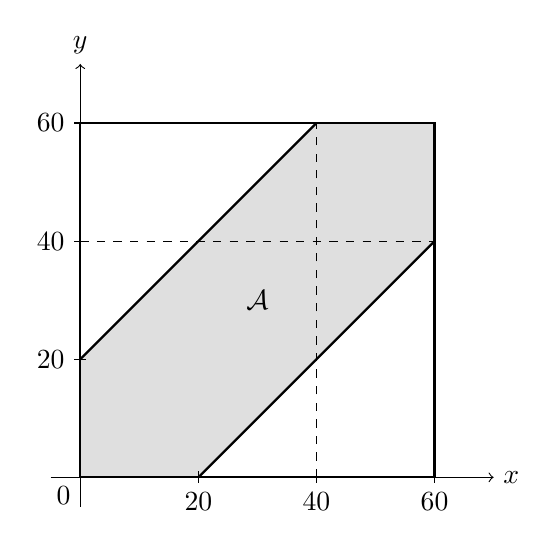
\begin{tikzpicture}[x=0.075cm, y=0.075cm]
            \fill[gray!25]
                (0,0) -- (20,0) -- (60,40) --
                (60,60) -- (40,60) -- (0,20) -- cycle;

            \draw[thick] (0,0) rectangle (60,60);
            \draw[thick] (0,20) -- (40,60);
            \draw[thick] (20,0) -- (60,40);

            \draw[dashed] (0,40) -- (60,40);
            \draw[dashed] (40,0) -- (40,60);

            \draw[->] (-5,0) -- (70,0) node[right] {$x$};
            \draw[->] (0,-5) -- (0,70) node[above] {$y$};

            \node[below left] at (0,0) {$0$};
            \foreach \t in {20,40,60} {
                \draw (\t,1) -- (\t,-1) node[below] {$\t$};
                \draw (1,\t) -- (-1,\t) node[left] {$\t$};
            }

            \node at (30,30) {$\mathcal{A}$};
        \end{tikzpicture}
    \end{center}

    \[
        \Pr(\mathcal{A})
        = \frac{S(\mathcal{A})}{S(\Omega)}
        = \frac{60^2 - 2 \cdot \frac{40^2}{2}}{3600}
        = \frac{2000}{3600}
        = \frac{5}{9}.
    \]
\end{example}

\begin{exercise}[Замечание]
    $\mathcal{F}$ - множество подмножеств $\Omega$, для которых определена $S$ (площадь)
\end{exercise}


\section{Свойства вероятности и основные формулы}
\subsection{$\sigma$ Аддитивность}
\begin{definition}
    Если мы возьмем счетный набор событий $\mathcal{A}_1, \mathcal{A}_2, \dots \mathcal{A}_n\in \mathcal{F}$, (счетное количество событий)\\
    причем дизъюнктивное объединение тоже является событием
    \[
        \mathcal{A} = \bigsqcup_{i=1}^{\infty} \mathcal{A}_i \in \mathcal{F}
    \]
    тогда 
    \[
    \Pr(\mathcal{A})
    =
    \Pr\left(\bigsqcup_{i=1}^{\infty} \mathcal{A}_i\right)
    =
    \Sum{i=1}{\infty} \Pr(\mathcal{A}_i).
    \]
    Это счетная сумма (аддитивность).
\end{definition}

\begin{exercise}[Замечание]
        Обычная аддитивность
        \[
    \Pr\left(\mathcal{A}_1 \sqcup \dots \sqcup \mathcal{A}_n\right)
    =
    \Pr(\mathcal{A}_1) + \dots + \Pr(\mathcal{A}_n).
\]
\end{exercise}

\subsection{Условная вероятность}
\begin{definition}
    Пусть $\mathcal{A}, \mathcal{B} \in \mathcal{F}$
    и $\Pr(\mathcal{B}) \neq 0$.
    Условной вероятностью события $\mathcal{A}$
    при условии события $\mathcal{B}$ называется число
    \[
        \Pr(\mathcal{A} \mid \mathcal{B})
        =
        \frac{\Pr(\mathcal{A} \cap \mathcal{B})}{\Pr(\mathcal{B})}.
    \]
\end{definition}

\begin{Proof}[Обоснование в классической модели.]

Пусть $\Pr(\mathcal{B}) > 0$. Если известно, что событие
$\mathcal{B}$ произошло, то остаются только исходы из
$\mathcal{B}$, которые по-прежнему равновероятны.
Из них событию $\mathcal{A}$ благоприятствуют исходы
из $\mathcal{A} \cap \mathcal{B}$. Поэтому
\[
    \Pr(\mathcal{A} \mid \mathcal{B})
    =
    \frac{|\mathcal{A} \cap \mathcal{B}|}{|\mathcal{B}|}
    =
    \frac{
        |\mathcal{A} \cap \mathcal{B}| / |\Omega|
    }{
        |\mathcal{B}| / |\Omega|
    }
    =
    \frac{\Pr(\mathcal{A} \cap \mathcal{B})}{\Pr(\mathcal{B})}.
\]
\end{Proof}

\begin{center}
    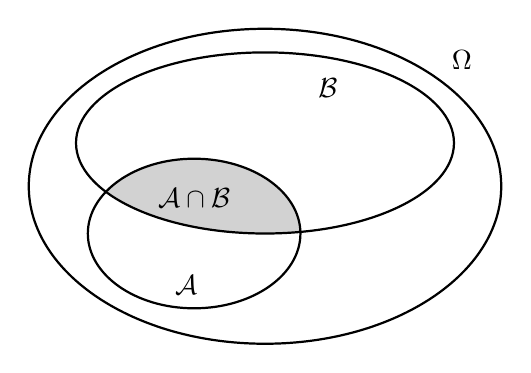
\begin{tikzpicture}[scale=1]
        % Пространство элементарных исходов.
        \draw[thick] (0,0) ellipse (3cm and 2cm);
        \node at (2.5,1.6) {$\Omega$};

        % Пересечение событий.
        \begin{scope}
            \clip (-0.9,-0.6) ellipse (1.35cm and 0.95cm);
            \fill[gray!35] (0,0.55) ellipse (2.4cm and 1.15cm);
        \end{scope}

        % События.
        \draw[thick]
            (-0.9,-0.6) ellipse (1.35cm and 0.95cm);
        \draw[thick]
            (0,0.55) ellipse (2.4cm and 1.15cm);

        \node at (-1,-1.25) {$\mathcal{A}$};
        \node at (0.8,1.25) {$\mathcal{B}$};
        \node at (-0.9,-0.15) {$\mathcal{A}\cap\mathcal{B}$};
    \end{tikzpicture}
\end{center}

\begin{example}[Пример: Условная вероятность при броске двух костей]
    Бросаются две игральные кости
    Обозначим через $\Sigma$ сумму выпавших очков

    Если $\Sigma = 6$, возможны исходы
    \[
        \{(1,5),(2,4),(3,3),(4,2),(5,1)\}.
    \]

    
    \[
        \Pr(\text{есть двойка} \mid \Sigma = 6)
        =
        \frac{
            \Pr\left(\{(2,4),(4,2)\}\right)
        }{
            \Pr\left(\{(1,5),(2,4),(3,3),(4,2),(5,1)\}\right)
        }
        =
        \frac{2/36}{5/36}
        =
        \frac{2}{5}.
    \]

    Если $\Sigma = 4$, возможны исходы
    \[
        \{(1,3),(2,2),(3,1)\}.
    \]
    
    
    \[
        \Pr(\text{есть двойка} \mid \Sigma = 4)
        =
        \frac{
            \Pr\left(\{(2,2)\}\right)
        }{
            \Pr\left(\{(1,3),(2,2),(3,1)\}\right)
        }
        =
        \frac{1/36}{3/36}
        =
        \frac{1}{3}.
    \]
\end{example}

\subsection{Формула полной вероятности}
\begin{definition}
    Пусть $\mathcal{A}_1, \mathcal{A}_2, \dots \mathcal{A}_n\in \mathcal{F}$, причем
    \[
        \Pr(\mathcal{A}_k) \neq 0, \qquad
        \
        \qquad
        \bigsqcup_{k=1}^{\infty} \mathcal{A}_k = \Omega.
    \]
    Тогда
    \[
        \Pr(\mathcal{B})
        =
        \sum_{k=1}^{\infty}
        \Pr(\mathcal{B} \mid \mathcal{A}_k) \cdot
        \Pr(\mathcal{A}_k).
    \]
\end{definition}
\begin{example}[Пример]
    Есть две урны:
    \begin{itemize}
        \item в первой --- 3 красных и 2 чёрных шара;
        \item во второй --- 1 красный и 4 чёрных шара.
    \end{itemize}
    Сначала равновероятно выбирают одну из урн, затем
    случайно вытаскивают из неё один шар.
    Найти вероятность того, что шар красный.
\end{example}

\begin{solution}
    Обозначим события:
    \[
        \mathcal{A}_1 = \{\text{выбрана первая урна}\},
        \qquad
        \mathcal{A}_2 = \{\text{выбрана вторая урна}\},
    \]
    \[
        \mathcal{B} = \{\text{вытащен красный шар}\}.
    \]
    События $\mathcal{A}_1$ и $\mathcal{A}_2$ несовместны
    и образуют полную группу:
    \[
        \mathcal{A}_1 \sqcup \mathcal{A}_2 = \Omega,
        \qquad
        \Pr(\mathcal{A}_1) = \Pr(\mathcal{A}_2) = \frac{1}{2}.
    \]
    Условные вероятности вытащить красный шар:
    \[
        \Pr(\mathcal{B} \mid \mathcal{A}_1) = \frac{3}{5},
        \qquad
        \Pr(\mathcal{B} \mid \mathcal{A}_2) = \frac{1}{5}.
    \]
    По формуле полной вероятности:
    \[
        \begin{aligned}
            \Pr(\mathcal{B})
            &=
            \Pr(\mathcal{B} \mid \mathcal{A}_1)
            \cdot \Pr(\mathcal{A}_1)
            +
            \Pr(\mathcal{B} \mid \mathcal{A}_2)
            \cdot \Pr(\mathcal{A}_2)
            \\
            &=
            \frac{3}{5} \cdot \frac{1}{2}
            +
            \frac{1}{5} \cdot \frac{1}{2}
            =
            \frac{2}{5}.
        \end{aligned}
    \]
\end{solution}


\subsection{Формула умножения вероятности}
\begin{definition}
    3 красных, 4 черных шариков, вытаскиваем последовательно
    \[
        \Pr(\text{черный -> черный -> красный}) = \frac{4}{7} \cdot \frac{3}{6} \cdot \frac{3}{5}
    \]

\end{definition}

\begin{Proof}
    Пусть $\Pr(\mathcal{A}_1 \cap \dots \cap \mathcal{A}_{n-1}) > 0$.
    По определению условной вероятности:
    \[
        \Pr(B \mid A)
        =
        \frac{\Pr(A \cap B)}{\Pr(A)}
        \implies
        \Pr(A \cap B) = \Pr(A)\Pr(B \mid A).
    \]
    Последовательно применяя эту формулу, получаем
    \[
        \begin{aligned}
            &\Pr(\mathcal{A}_1 \cap \dots \cap \mathcal{A}_n)
            \\
            &=
            \Pr(\mathcal{A}_1 \cap \dots \cap \mathcal{A}_{n-1})
            \Pr(\mathcal{A}_n \mid
                \mathcal{A}_1 \cap \dots \cap \mathcal{A}_{n-1})
            \\
            &= \dots =
            \Pr(\mathcal{A}_1)
            \Pr(\mathcal{A}_2 \mid \mathcal{A}_1)
            \cdot \ldots \cdot
            \Pr(\mathcal{A}_n \mid
                \mathcal{A}_1 \cap \dots \cap \mathcal{A}_{n-1}).
        \end{aligned}
    \]
    При подстановке условных вероятностей дробями
    множители последовательно сокращаются:
    \[
        \begin{aligned}
            &\Pr(\mathcal{A}_1)
            \cdot
            \frac{\Pr(\mathcal{A}_1 \cap \mathcal{A}_2)}
                 {\Pr(\mathcal{A}_1)}
            \cdot \ldots \cdot
            \frac{\Pr(\mathcal{A}_1 \cap \dots \cap \mathcal{A}_n)}
                 {\Pr(\mathcal{A}_1 \cap \dots \cap \mathcal{A}_{n-1})}
            \\
            &= \Pr(\mathcal{A}_1 \cap \dots \cap \mathcal{A}_n).
        \end{aligned}
    \]
\end{Proof}
\subsection{Формула Байеса}

\begin{theorem}[Формула Байеса]
    Пусть события $\mathcal{B}_1,\mathcal{B}_2,\dots$
    :
    \[
        \bigsqcup_{i=1}^{\infty} \mathcal{B}_i = \Omega,
        \qquad
        \Pr(\mathcal{B}_i) \neq 0.
    \]
    Тогда для события $\mathcal{A}$, такого что
    $\Pr(\mathcal{A}) \neq 0$, выполняется
    \[
        \Pr(\mathcal{B}_k \mid \mathcal{A})
        =
        \frac{\Pr(\mathcal{A} \cap \mathcal{B}_k)}
             {\Pr(\mathcal{A})}
        =
        \frac{
            \Pr(\mathcal{A} \mid \mathcal{B}_k)
            \cdot \Pr(\mathcal{B}_k)
        }{
            \Sum{i=1}{\infty}
            \Pr(\mathcal{A} \mid \mathcal{B}_i)
            \cdot \Pr(\mathcal{B}_i)
        }.
    \]
    Для конечной полной группы из $n$ событий
    $\Sigma$ берётся от $1$ до $n$.
\end{theorem}

\subsection{Независимость событий}

\begin{definition}
    События $\mathcal{A}, \mathcal{B} \in \mathcal{F}$
    называются \textbf{независимыми}, если
    \[
        \Pr(\mathcal{A} \cap \mathcal{B})
        =
        \Pr(\mathcal{A}) \cdot \Pr(\mathcal{B}).
    \]
    Обозначение:
    \[
        \mathcal{A} \perp\!\!\!\perp \mathcal{B}.
    \]
    Если $\Pr(\mathcal{B}) > 0$, это равносильно условию
    \[
        \Pr(\mathcal{A} \mid \mathcal{B})
        =
        \frac{\Pr(\mathcal{A} \cap \mathcal{B})}{\Pr(\mathcal{B})}
        =
        \Pr(\mathcal{A}).
    \]
    То есть наступление события $\mathcal{B}$ не меняет
    вероятность события $\mathcal{A}$.
\end{definition}

\subsubsection{Попарная независимость и независимость в совокупности}

\begin{definition}[Попарная независимость]
    События $\mathcal{A}_1,\dots,\mathcal{A}_n$
    называются \textbf{попарно независимыми}, если
    \[
        \Pr(\mathcal{A}_i \cap \mathcal{A}_j)
        =
        \Pr(\mathcal{A}_i)\cdot\Pr(\mathcal{A}_j)
        \qquad
        \forall\,1 \leq i < j \leq n.
    \]
\end{definition}





\begin{definition}[Независимость в совокупности]
    События $\mathcal{A}_1,\dots,\mathcal{A}_n$
    называются \textbf{независимыми в совокупности}, если
    для любого $k \in \{2,\dots,n\}$ и любых индексов
    \[
        1 \leq i_1 < i_2 < \dots < i_k \leq n
    \]
    выполняется
    \[
        \Pr(\mathcal{A}_{i_1} \cap \dots \cap \mathcal{A}_{i_k})
        =
        \Pr(\mathcal{A}_{i_1})\cdot\ldots\cdot
        \Pr(\mathcal{A}_{i_k}).
    \]
    То есть равенство проверяется для любой выбранной группы
    событий, а не только для пар.
\end{definition}

\begin{exercise}[Замечание]
    Из независимости в совокупности следует попарная независимость.
    Обратное утверждение в общем случае неверно.
\end{exercise}

\begin{example}[Пример Бернштейна]
    Равновероятно выбирается одна из четырёх вершин тетраэдра
    \begin{center}
        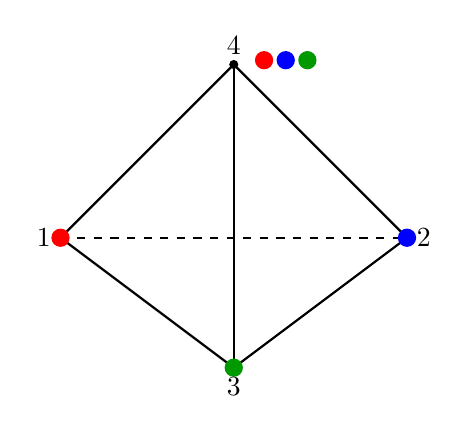
\begin{tikzpicture}[scale=1.1]
            \coordinate (v1) at (-2,0);
            \coordinate (v2) at (2,0);
            \coordinate (v3) at (0,-1.5);
            \coordinate (v4) at (0,2);

            \draw[thick] (v1) -- (v4) -- (v2) -- (v3) -- cycle;
            \draw[thick] (v4) -- (v3);
            \draw[thick,dashed] (v1) -- (v2);

            \fill[red] (v1) circle (3pt);
            \fill[blue] (v2) circle (3pt);
            \fill[green!60!black] (v3) circle (3pt);
            \fill (v4) circle (1.5pt);

            \node[left] at (v1) {$1$};
            \node[right] at (v2) {$2$};
            \node[below] at (v3) {$3$};
            \node[above] at (v4) {$4$};

            \fill[red] (0.35,2.05) circle (3pt);
            \fill[blue] (0.60,2.05) circle (3pt);
            \fill[green!60!black] (0.85,2.05) circle (3pt);
        \end{tikzpicture}
    \end{center}

    Получаем классическую модель:
    \[
        \Omega = \{\omega_1,\omega_2,\omega_3,\omega_4\},
        \qquad
        \Pr(\{\omega_i\}) = \frac14.
    \]
    Рассмотрим события:
    \[
        \begin{aligned}
            \mathcal{A}_1
            &= \{\text{выбранная вершина имеет красную отметку}\}
            = \{\omega_1,\omega_4\},\\
            \mathcal{A}_2
            &= \{\text{выбранная вершина имеет синюю отметку}\}
            = \{\omega_2,\omega_4\},\\
            \mathcal{A}_3
            &= \{\text{выбранная вершина имеет зелёную отметку}\}
            = \{\omega_3,\omega_4\}.
        \end{aligned}
    \]
    Каждое событие содержит два исхода, поэтому
    \[
        \Pr(\mathcal{A}_1)
        =
        \Pr(\mathcal{A}_2)
        =
        \Pr(\mathcal{A}_3)
        =
        \frac12.
    \]

    \[
        \Pr(\mathcal{A}_i \cap \mathcal{A}_j)
        =
        \frac14
        =
        \frac12 \cdot \frac12
        =
        \Pr(\mathcal{A}_i)\Pr(\mathcal{A}_j),
        \qquad i \neq j.
    \]
    Следовательно, события попарно независимы.

    \[
        \Pr(\mathcal{A}_1 \cap \mathcal{A}_2 \cap \mathcal{A}_3)
        =
        \frac14
        \neq
        \frac18
        =
        \Pr(\mathcal{A}_1)\Pr(\mathcal{A}_2)\Pr(\mathcal{A}_3).
    \]
    Независимости в совокупности нет.
\end{example}




\begin{example}[Пример: Формула умножения и независимость событий. Как их правильно отличать?]
    В урне 3 красных и 4 чёрных шара. Последовательно
    вытаскивают два шара. Обозначим события
    \[
        \mathcal{A} = \{\text{первый шар чёрный}\},
        \qquad
        \mathcal{B} = \{\text{второй шар чёрный}\}.
    \]

    \textbf{1. Без возвращения.}

    Если первый шар оказался чёрным, в урне осталось
    3 чёрных шара из 6. Поэтому
    \[
        \Pr(\mathcal{B} \mid \mathcal{A}) = \frac{3}{6}.
    \]
    По формуле полной вероятности
    \[
        \Pr(\mathcal{B})
        =
        \frac{4}{7} \cdot \frac{3}{6}
        +
        \frac{3}{7} \cdot \frac{4}{6}
        =
        \frac{4}{7}.
    \]
    Следовательно,
    \[
        \Pr(\mathcal{B} \mid \mathcal{A})
        \neq
        \Pr(\mathcal{B}),
    \]
    то есть события зависимы. По формуле умножения:
    \[
        \Pr(\mathcal{A} \cap \mathcal{B})
        =
        \Pr(\mathcal{A})
        \cdot \Pr(\mathcal{B} \mid \mathcal{A})
        =
        \frac{4}{7} \cdot \frac{3}{6}
        =
        \frac{2}{7}.
    \]

    \textbf{2. С возвращением и перемешиванием.}

    Первый шар возвращают в урну и перемешивают её содержимое.
    Перед вторым вытаскиванием состав урны прежний,
    поэтому события независимы:
    \[
        \Pr(\mathcal{B} \mid \mathcal{A})
        =
        \Pr(\mathcal{B})
        =
        \frac{4}{7}.
    \]
    Формула умножения принимает вид
    \[
        \Pr(\mathcal{A} \cap \mathcal{B})
        =
        \Pr(\mathcal{A}) \cdot \Pr(\mathcal{B})
        =
        \frac{4}{7} \cdot \frac{4}{7}
        =
        \frac{16}{49}.
    \]

    Формула умножения применима в обоих случаях.
    Независимость позволяет заменить условную вероятность
    $\Pr(\mathcal{B} \mid \mathcal{A})$ на $\Pr(\mathcal{B})$.
\end{example}

\section{Системы множеств}

\subsection{Полукольцо}
\begin{definition}
    Система множеств $S$ называется полукольцом, если
    \begin{enumerate}[label=\arabic*)]
        \item $\varnothing \in S$
        \item $A, B \in S,\text{ то }  A \cap B \in S $ - Замкнутость относительно операции пересечения
        \item $A, B \in S \text{, то  } \exists A_1, ..., A_n \in S:$
        \\
        A $\setminus$ B = $\bigsqcup_{i=1}^{n} \mathcal{A}_i$
        
        
    \end{enumerate}
\end{definition}
\begin{example}
    Промежутки на $\mathbb{R}$
    Рассмотрим систему $S$ всех промежутков на $\mathbb{R}$, \\
    Проверим свойства полукольца

    \begin{enumerate}[label=\arabic*)]
        \item $S \neq \varnothing$, поскольку, например, $[0;8] \in S$.

        \item Пересечение двух промежутков является промежутком
        либо пустым множеством. Следовательно,
        \[
            A, B \in S \implies A \cap B \in S.
        \]

        \item Разность двух промежутков представляется
        как объединение не более двух непересекающихся
        промежутков.

        Например, пусть
        \[
            A = [0;8], \qquad B = [1;3).
        \]
        Тогда
        \[
            A \setminus B = [0;1) \sqcup [3;8]
        \]
        

        Обозначив
        \[
            A_1 = [0;1), \qquad A_2 = [3;8],
        \]
        получаем
        \[
            A \setminus B = A_1 \sqcup A_2,
            \qquad A_1, A_2 \in S,
            \qquad A_1 \cap A_2 = \varnothing.
        \]
    \end{enumerate}

    Таким образом, система $S$ является полукольцом
\end{example}

\subsubsection{Симметрическая разность}

\begin{definition}
    Симметрической разностью множеств $A$ и $B$
    называется множество элементов, принадлежащих
    ровно одному из этих множеств:
    \[
        A \triangle B
        =
        (A \cup B) \setminus (A \cap B)
        =
        (A \setminus B) \sqcup (B \setminus A).
    \]
\end{definition}

% В преамбулу: \usepackage{tikz}
\begin{center}
    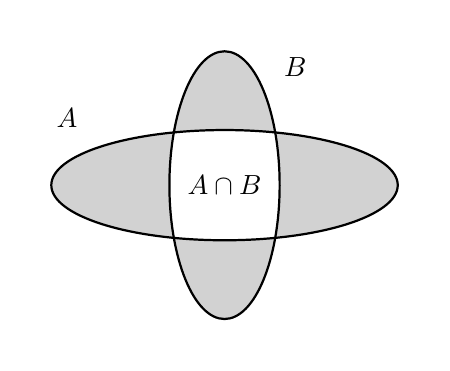
\begin{tikzpicture}
        \begin{scope}
            \clip (-2.5,-2) rectangle (2.5,2);
            \fill[gray!35, even odd rule]
                (0,0) ellipse (2.2cm and 0.7cm)
                (0,0) ellipse (0.7cm and 1.7cm);
        \end{scope}

        \draw[thick] (0,0) ellipse (2.2cm and 0.7cm);
        \draw[thick] (0,0) ellipse (0.7cm and 1.7cm);

        \node at (-2,0.85) {$A$};
        \node at (0.9,1.5) {$B$};
        \node at (0,0) {$A \cap B$};
    \end{tikzpicture}
\end{center}
\subsection{Кольцо}
\begin{definition}
    Система множеств $R$ называется \textbf{кольцом}, если
    \begin{enumerate}[label=\arabic*)]
        \item $\varnothing \neq R$;
        \item $\forall$ $A, B \in R$ выполняется
        \[
            A \cap B \in R,
            \qquad
            A \triangle B \in R.
        \]
    \end{enumerate}
\end{definition}
\begin{exercise}[Замечание]
        Кольцо замкнуто относительно всех операций
    \[
        A, B \in R
        \implies
        A \cup B \in R,
        \qquad
        A \setminus B \in R
    \]
    
    \begin{center}
        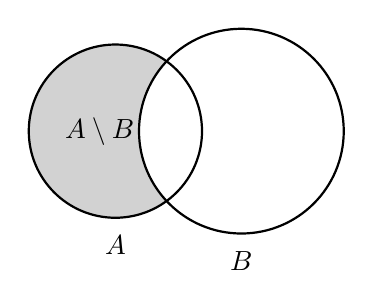
\begin{tikzpicture}
    
            \begin{scope}
                \clip (-0.8,0) circle (1.1cm);
                \fill[gray!35, even odd rule]
                    (-3,-2) rectangle (3,2)
                    (0.8,0) circle (1.3cm);
            \end{scope}

            \draw[thick] (-0.8,0) circle (1.1cm);
            \draw[thick] (0.8,0) circle (1.3cm);

            \node at (-0.8,-1.45) {$A$};
            \node at (0.8,-1.65) {$B$};
            \node at (-1,0) {$A \setminus B$};
        \end{tikzpicture}
    \end{center}
\end{exercise}

\begin{exercise}[Замечание]
    Любое кольцо является полукольцом.
    Проверим условия:
    \begin{enumerate}[label=\arabic*)]
        \item $\varnothing \in R$, поэтому $R \neq \varnothing$.

        \item Если $A, B \in R$, то $A \cap B \in R$ - верно

        \item Если $A, B \in R$, то $A \setminus B \in R$.
        Поэтому достаточно взять $A_1 = A \setminus B$:
        \[
            A \setminus B = \bigsqcup_{i=1}^{1} A_i,
            \qquad A_1 \in R.
        \]
    \end{enumerate}
\end{exercise}

\begin{exercise}[Замечание]
    Пусть $S = \{A_\alpha\}_{\alpha \in I}$ --- полукольцо.
    Положим
    \[
        \Omega = \bigcup_{\alpha \in I} A_\alpha.
    \]
    Тогда
    \[
        S \subset 2^\Omega.
    \]
    В частности, существует кольцо $R$, содержащее $S$:
    можно взять $R = 2^\Omega$
    \[
        S \subset R = 2^\Omega.
    \]
    Вывод: если есть полукольцо, всегда есть кольцо, которое содержит данное полукольцо
\end{exercise}

\subsection{Наименьшее кольцо}
\begin{definition}
    Пусть $\chi$ --- система множеств.
    Кольцо $R(\chi)$ называется \textbf{наименьшим кольцом,
    содержащим $\chi$}, если
    \begin{enumerate}[label=\arabic*)]
        \item $\chi \subset R(\chi)$;
        \item $\forall$ $R_1$, кольца: если $\chi$ $\subset$ $R_1$, то верно
        \[
            R(\chi) \subset R_1.
        \]
    \end{enumerate}

\end{definition}

\subsubsection{Существование наименьшего кольца}

\begin{theorem}
    Для любой системы множеств $\chi$ существует
    наименьшее кольцо $R(\chi)$, содержащее $\chi$
\end{theorem}

\begin{Proof}
    \begin{enumerate}[label=\arabic*)]
        \item Хотя бы одно кольцо, содержащее $\chi$, существует:
        \[
            \Omega = \bigcup_{A_i \in \chi} A_i,
            \qquad R_1 = 2^\Omega
        \]

        \item Рассмотрим все кольца подмножеств $\Omega$,
        содержащие $\chi$, и обозначим их
        $\{R_\alpha\}_{\alpha \in I}$. Положим
        \[
            R(\chi) = \bigcap_{\alpha \in I} R_\alpha
        \]
        Проверим свойства $R(\chi)$.
    \end{enumerate}

    \textbf{I. $R(\chi)$ --- кольцо.}
    \begin{enumerate}[label=\arabic*)]
        \item Поскольку $\varnothing \in R_\alpha$
        для каждого $\alpha \in I$, имеем
        \[
            \varnothing \in
            \bigcap_{\alpha \in I} R_\alpha = R(\chi).
        \]

        \item Пусть $A, B \in R(\chi)$. Тогда
        \[
            A, B \in R_\alpha
            \qquad \forall \alpha \in I.
        \]
        Каждая система $R_\alpha$ является кольцом, поэтому
        \[
            A \cap B \in R_\alpha,
            \qquad
            A \triangle B \in R_\alpha
            \qquad \forall \alpha \in I.
        \]
        Следовательно,
        \[
            A \cap B \in R(\chi),
            \qquad
            A \triangle B \in R(\chi).
        \]
    \end{enumerate}

    \textbf{II. $\chi \subset R(\chi)$}

    Поскольку $\chi \subset R_\alpha$ для каждого $\alpha \in I$,
    \[
        \chi \subset \bigcap_{\alpha \in I} R_\alpha = R(\chi).
    \]

    \textbf{III. $R(\chi)$ --- наименьшее такое кольцо.}

Пусть $R_0$ --- произвольное кольцо, содержащее $\chi$:
\[
    \chi \subset R_0.
\]
Рассмотрим
\[
    R_0' = \{A \in R_0 \colon A \subset \Omega\}.
\]
Тогда $\chi \subset R_0'$. Если $A,B \in R_0'$, то
\[
    A=A_0,\quad B=B_0,\qquad
    A_0,B_0\in R_0,\quad A_0,B_0\subset\Omega.
\]
Поэтому
\[
    A\cap B=(A_0\cap B_0)\cap\Omega\in R_0',
\]
\[
    A\triangle B
    =(A_0\cap\Omega)\triangle(B_0\cap\Omega)
    =(A_0\triangle B_0)\cap\Omega\in R_0',
\]
так как $A_0\triangle B_0\in R_0$ и
$A_0\triangle B_0\subset\Omega$.
Следовательно, $R_0'$ --- кольцо подмножеств $\Omega$,
содержащее $\chi$, то есть
\[
    \exists \alpha_0 \in I \colon R_0' = R_{\alpha_0}.
\]
Следовательно,
\[
    R(\chi) = \bigcap_{\alpha \in I} R_\alpha
    \subset R_{\alpha_0} = R_0' \subset R_0.
\]
\end{Proof}

\subsection{Наименьшее кольцо, содержащее полукольцо}
\begin{theorem}
    Пусть $S$ --- полукольцо. Тогда
    \[
        R(S)
        =
        \left\{
            \bigsqcup_{i=1}^{n} A_i
            \;\middle|\;
            n \in \mathbb{N},\;
            A_i \in S\;
        \right\}.
    \]
\end{theorem}
\begin{Proof}
    Обозначим множество из правой части как $K = \left\{ \bigsqcup_{i=1}^{n} A_i \;\middle|\; A_i \in S \right\}$. 
    Нам нужно доказать два включения: $K \subset R(S)$ и $R(S) \subset K$. %[cite: 9]

    \textbf{1. Включение $K \subset R(S)$.} \\
    Возьмем произвольный элемент $x \in K$. По определению множества $K$, $x$ представим в виде дизъюнктного объединения конечного числа элементов полукольца:
    \[
        x = \bigsqcup_{i=1}^{n} A_i, \quad A_i \in S.
    \]
    Поскольку $S \subset R(S)$ (по определению наименьшего кольца), каждый $A_i \in R(S)$. Так как $R(S)$ --- кольцо, оно замкнуто относительно конечных объединений, следовательно, $x \in R(S)$. Включение доказано. %[cite: 9]

    \textbf{2. Включение $R(S) \subset K$.} \\
    Чтобы доказать это включение, достаточно показать, что $K$ само является кольцом. Так как $K$ содержит $S$ (достаточно взять $n=1$), а $R(S)$ --- \textit{наименьшее} кольцо, содержащее $S$, из того, что $K$ --- кольцо, мгновенно последует $R(S) \subset K$. %[cite: 9]
    
    Для доказательства того, что $K$ --- кольцо, нам понадобится вспомогательная лемма.
\end{Proof}

\subsection{Лемма о разности элементов полукольца}

\begin{lemma}
    Если $A, B_1, B_2, \dots, B_m \in S$, то существуют такие $A_1, A_2, \dots, A_n \in S$, что:
    \[
        A \setminus B_1 \setminus B_2 \setminus \dots \setminus B_m = \bigsqcup_{i=1}^{n} A_i.
    \]
\end{lemma}

\begin{Proof}[Доказательство леммы]
    Доказывать будем по индукции по $m$. %[cite: 9]
    
    \textbf{База индукции ($m=1$):} \\
    Утверждение $A \setminus B_1 = \bigsqcup_{i=1}^{n} A_i$ выполняется по определению полукольца (свойство разности). %[cite: 9]

    \textbf{Шаг индукции:} \\
    Пусть утверждение верно для $m$. Докажем для $m+1$. %[cite: 9]
    \[
        A \setminus B_1 \setminus \dots \setminus B_m \setminus B_{m+1} = \left( \bigsqcup_{i=1}^{n} A_i \right) \setminus B_{m+1} = \bigsqcup_{i=1}^{n} (A_i \setminus B_{m+1}).
    \]
    Так как $A_i \in S$ и $B_{m+1} \in S$, по определению полукольца разность $A_i \setminus B_{m+1}$ представима в виде $\bigsqcup_{j=1}^{k_i} C_{ij}$, где $C_{ij} \in S$. %[cite: 9]
    Тогда:
    \[
        \bigsqcup_{i=1}^{n} (A_i \setminus B_{m+1}) = \bigsqcup_{i=1}^{n} \left( \bigsqcup_{j=1}^{k_i} C_{ij} \right) = \bigsqcup_{i, j} C_{ij}.
    \]
    Получили дизъюнктивное объединение конечного числа элементов из $S$. Лемма доказана. %[cite: 9]
\end{Proof}

\begin{Proof}[{{Продолжение доказательства теоремы (проверка, что $K$ --- кольцо)}}]
    \begin{enumerate}[label=\arabic*)]
        \item $\varnothing \in K$, так как $S \subset K$ и $\varnothing \in S$. %[cite: 10]
        \item Пусть $P, Q \in K$. Докажем, что $P \cap Q \in K$ и $P \triangle Q \in K$. %[cite: 10]
        
        По определению $K$, элементы $P$ и $Q$ имеют вид:
        \[
            P = \bigsqcup_{i=1}^{n} P_i, \quad Q = \bigsqcup_{j=1}^{m} Q_j, \qquad P_i, Q_j \in S.
        \]
        
        \textbf{Пересечение:}
        \[
            P \cap Q = \left( \bigsqcup_{i=1}^{n} P_i \right) \cap \left( \bigsqcup_{j=1}^{m} Q_j \right) = \bigsqcup_{i=1}^{n} \bigsqcup_{j=1}^{m} (P_i \cap Q_j).
        \]
        Обозначим $D_{ij} = P_i \cap Q_j$. Так как $S$ замкнуто относительно пересечений, $D_{ij} \in S$. Значит, $P \cap Q = \bigsqcup_{i,j} D_{ij} \in K$. %[cite: 10]

        \textbf{Симметрическая разность:} \\
        Рассмотрим сначала разность $P \setminus Q$: %[cite: 11]
        \[
            P \setminus Q = \left( \bigsqcup_{i=1}^{n} P_i \right) \setminus \left( \bigsqcup_{j=1}^{m} Q_j \right) = \bigsqcup_{i=1}^{n} (P_i \setminus Q_1 \setminus Q_2 \setminus \dots \setminus Q_m).
        \]
        По доказанной лемме, каждый элемент $P_i \setminus Q_1 \setminus \dots \setminus Q_m$ представим как $\bigsqcup_{\ell=1}^{W_i} F_{i\ell}$, где $F_{i\ell} \in S$. %[cite: 11]
        Отсюда $P \setminus Q = \bigsqcup_{i, \ell} F_{i\ell} \in K$.
        
        Аналогично расписывается $Q \setminus P$:
        \[
            Q \setminus P = \bigsqcup_{j=1}^{m} (Q_j \setminus P_1 \setminus \dots \setminus P_n) = \bigsqcup_{j=1}^{m} \bigsqcup_{k=1}^{T_j} E_{jk} \in K, \quad E_{jk} \in S. %[cite: 11]
        \]
        
        Тогда симметрическая разность:
        \[
            P \triangle Q = (P \setminus Q) \sqcup (Q \setminus P) = \left( \bigsqcup_{i, \ell} F_{i\ell} \right) \sqcup \left( \bigsqcup_{j, k} E_{jk} \right) \in K. %[cite: 11]
        \]
    \end{enumerate}
    Мы доказали, что $K$ --- кольцо. Следовательно, $R(S) = K$. Теорема полностью доказана. %[cite: 11]
\end{Proof}

\subsection{$\sigma$-кольца и $\delta$-кольца}

\begin{definition}[$\delta$-кольцо]
    $\delta$-кольцом называется кольцо, замкнутое относительно счетного пересечения:
    \[
        A_1, A_2, \dots \in R \implies \bigcap_{i=1}^{\infty} A_i \in R.
    \] %[cite: 12]
\end{definition}

\begin{definition}[$\sigma$-кольцо]
    $\sigma$-кольцом называется кольцо, замкнутое относительно счетного объединения:
    \[
        A_1, A_2, \dots \in R \implies \bigcup_{i=1}^{\infty} A_i \in R.
    \] %[cite: 12]
\end{definition}

\begin{exercise}[Свойство вложенности]
    Любое $\sigma$-кольцо является $\delta$-кольцом ($\sigma\text{-кольцо} \implies \delta\text{-кольцо}$). %[cite: 12]
\end{exercise}

\begin{Proof}
    Пусть $R$ --- $\sigma$-кольцо и $A_1, A_2, \dots \in R$. Рассмотрим их счетное пересечение. Воспользуемся законами де Моргана: %[cite: 12]
    \[
        \bigcap_{i=1}^{\infty} A_i = \bigcap_{i=1}^{\infty} (A_1 \cap A_i) = A_1 \setminus \left( A_1 \setminus \bigcap_{i=2}^{\infty} A_i \right) = A_1 \setminus \bigcup_{i=2}^{\infty} (A_1 \setminus A_i).
    \]
    Проанализируем правую часть: %[cite: 12]
    \begin{itemize}
        \item $A_1 \setminus A_i \in R$, так как $R$ --- кольцо (замкнуто относительно разности).
        \item $\bigcup_{i=2}^{\infty} (A_1 \setminus A_i) \in R$, так как $R$ --- $\sigma$-кольцо (замкнуто относительно счетного объединения).
        \item Итоговая разность $A_1 \setminus \left( \dots \right)$ также принадлежит $R$, так как кольцо замкнуто относительно разности.
    \end{itemize}
    Следовательно, $\bigcap_{i=1}^{\infty} A_i \in R$, что и требовалось доказать. %[cite: 12]
\end{Proof}

\begin{example}
    Обратное утверждение неверно: $\delta$-кольцо $\not\implies$ $\sigma$-кольцо. %[cite: 12]
    \\
    \\
    В качестве контрпримера рассмотрим систему всех ограниченных подмножеств $\R$. %[cite: 12] 
    Эта система образует $\delta$-кольцо, поскольку пересечение любого (в том числе счетного) числа ограниченных множеств остается ограниченным. Однако она не является $\sigma$-кольцом: счетное объединение ограниченных множеств может дать неограниченное множество. 
\end{example}

\subsection{Полуалгебра и алгебра}

\begin{definition}[Единица системы множеств]
    Множество $X \in S$ называется \textbf{единицей}
    системы множеств $S$, если
    \[
        A \subset X \qquad \forall A \in S.
    \]
\end{definition}

\begin{definition}[Полуалгебра]
    \textbf{Полуалгебра} --- это полукольцо с единицей.
\end{definition}

\begin{definition}[Алгебра]
    \textbf{Алгебра} --- это кольцо с единицей.
\end{definition}

% Продолжение по лекциям 7--10: материал сгруппирован по темам.
% Источник: лекция 8, с. 5--8; лекция 9, с. 9;
% лекция 10, с. 15--18 рукописного PDF.

\subsection{Счётные операции над множествами}

\begin{center}
    \begin{tikzpicture}[>=Stealth, every node/.style={font=\small}]
        \node (s) at (0,0) {Полукольцо};
        \node (r) at (3,0) {Кольцо};
        \node (sr) at (6.1,0.35) {$\sigma$-кольцо};
        \node (dr) at (6.1,-0.55) {$\delta$-кольцо};
        \draw[->] (s) -- (r);
        \draw[->] (r) -- (4.6,0) |- (sr);
        \draw[->] (4.6,0) |- (dr);
        \draw[->] (sr) -- (dr);
        \node (sa) at (0,-1.65) {Полуалгебра};
        \node (a) at (3,-1.65) {Алгебра};
        \node (sigma) at (6.1,-1.65) {$\sigma$-алгебра};
        \node (delta) at (6.1,-2.65) {$\delta$-алгебра};
        \draw[->] (sa) -- (a);
        \draw[->] (a) -- (sigma);
        \node at (6.1,-2.15) {$\Updownarrow$};
    \end{tikzpicture}
\end{center}

\begin{definition}[$\sigma$-алгебра с единицей $\Omega$]
    Система $\mathcal{F} \subset 2^\Omega$ называется
    \textbf{$\sigma$-алгеброй с единицей $\Omega$}, если
    \begin{enumerate}[label=\arabic*)]
        \item $\Omega \in \mathcal{F}$;
        \item $\mathcal{F}$ замкнута относительно операций
        $\cap$, $\cup$, $\setminus$, $\triangle$:
        \[
            A,B \in \mathcal{F}
            \implies A \star B \in \mathcal{F},
            \qquad \star \in \{\cap,\cup,\setminus,\triangle\};
        \]
        \item для любой последовательности $A_i \in \mathcal{F}$
        \[
            \bigcup_{i=1}^{\infty} A_i \in \mathcal{F}.
        \]
    \end{enumerate}
    При этом
    \[
        \varnothing = \Omega \setminus \Omega \in \mathcal{F},
        \qquad
        \bigcap_{i=1}^{\infty} B_i
        = \overline{\bigcup_{i=1}^{\infty}\overline{B_i}}
        \in \mathcal{F}
        \quad (B_i \in \mathcal{F}).
    \]
\end{definition}

\subsection{Наименьшая \texorpdfstring{$\sigma$}{σ}-алгебра}

\begin{definition}
    Пусть $\chi$ --- система множеств,
    $\Omega = \bigcup_{A\in\chi} A$.
    Наименьшая $\sigma$-алгебра $\sigma(\chi)$ определяется условиями:
    \begin{enumerate}[label=\arabic*)]
        \item $\chi \subset \sigma(\chi)$;
        \item $\sigma(\chi)$ --- $\sigma$-алгебра с единицей $\Omega$;
        \item для любой $\sigma$-алгебры $\mathcal{A}$
        с той же единицей $\Omega$
        \[
            \chi \subset \mathcal{A}
            \implies \sigma(\chi) \subset \mathcal{A}.
        \]
    \end{enumerate}
\end{definition}

\textbf{Построение:}
\[
    \sigma(\chi) = \bigcap_{\alpha} \mathcal{A}_\alpha,
\]
где $\mathcal{A}_\alpha$ --- все $\sigma$-алгебры
с единицей $\Omega$, содержащие $\chi$.

\subsection{Принцип подходящих множеств}

\begin{task}
    Для любого $A\in R(\chi)$ существует конечное покрытие
    элементами $\chi$:
    \[
        \exists A_1,\ldots,A_n\in\chi\colon
        A\subset\bigcup_{i=1}^{n} A_i.
    \]
\end{task}

\begin{solution}
    Рассмотрим
    \[
        R_0 = \left\{A\in R(\chi)\;\middle|\;
        \exists A_1,\ldots,A_n\in\chi\colon
        A\subset\bigcup_{i=1}^{n} A_i\right\}.
    \]
    Тогда
    \[
        R_0\subset R(\chi),\qquad
        \chi\subset R_0,\qquad R_0\text{ --- кольцо}.
    \]
    По минимальности $R(\chi)$:
    \[
        R(\chi)\subset R_0
        \quad\Longrightarrow\quad R_0=R(\chi).
    \]
\end{solution}

\[
    S\longrightarrow R(S)\longrightarrow\sigma(S),
    \qquad
    R(S)=\left\{\bigsqcup_{i=1}^{n}A_i\;\middle|\;
    n\in\N,\ A_i\in S\right\}.
\]

\subsection{Борелевская \texorpdfstring{$\sigma$}{σ}-алгебра}

\begin{definition}
    \textbf{Борелевской $\sigma$-алгеброй} на пространстве $A$
    называется наименьшая $\sigma$-алгебра, содержащая все
    открытые множества этого пространства.
    Обозначение: $\mathcal{B}(A)$.
\end{definition}

\subsubsection{Открытые множества на \texorpdfstring{$\mathbb{R}$}{R}}

\begin{theorem}
    Любое открытое множество $A\subset\R$ представляется
    в виде конечного или счётного дизъюнктного объединения
    открытых интервалов:
    \[
        A=\bigsqcup_{i\in I}(a_i;b_i),
        \qquad a_i,b_i\in\overline{\R},
    \]
    где $I$ --- не более чем счётное множество индексов.
\end{theorem}

\begin{Proof}
    Введём на $A$ отношение эквивалентности:
    \[
        x\sim y \quad\Longleftrightarrow\quad [x;y]\subset A.
    \]
    Здесь $[x;y]$ --- отрезок между $x$ и $y$.
    \begin{enumerate}[label=\arabic*)]
        \item Рефлексивность: $x\sim x$ для всех $x\in A$.
        \item Симметричность: $x\sim y\implies y\sim x$.
        \item Транзитивность:
        $x\sim y$, $y\sim z\implies x\sim z$.
    \end{enumerate}
    Разобьём $A$ на классы эквивалентности:
    \[
        A=\bigsqcup_{\alpha} A_\alpha.
    \]
    \textbf{1. $A_\alpha$ --- открытый интервал.}
    По определению отношения $A_\alpha$ является промежутком.
    Пусть, например, $A_\alpha=(a;b]$.
    Тогда $b\in A_\alpha\subset A$, поэтому
    существует $U_\eps(b)\subset A$.
    Пусть $(b;b+\eps)\subset A_\beta$.
    При достаточно малом $\eps>0$:
    \[
        b-\frac{\eps}{2}\sim b+\frac{\eps}{2},
    \]
    что противоречит тому, что $b$ --- правый конец $A_\alpha$.

    \textbf{2. Классов не более чем счётное число.}
    В каждом $(a_\alpha;b_\alpha)$ выберем рациональное число:
    \[
        q_\alpha\in\Q\cap(a_\alpha;b_\alpha).
    \]
    Интервалы не пересекаются, поэтому выбранные числа различны.
\end{Proof}

\subsubsection{Порождающие системы}

\begin{theorem}
    \[
        \begin{aligned}
            \mathcal{B}(\R)
            &=\sigma\bigl(\{(a;b)\}_{a,b\in\R}\bigr)
              =\mathcal{B}_2\\
            &=\sigma\bigl(\{[a;b]\}_{a,b\in\R}\bigr)
              =\mathcal{B}_3\\
            &=\sigma\bigl(\{(-\infty;x]\}_{x\in\R}\bigr)
              =\mathcal{B}_4\\
            &=\sigma\bigl(\{(a;b)\}_{a,b\in\Q}\bigr)
              =\mathcal{B}_5.
        \end{aligned}
    \]
\end{theorem}

\begin{Proof}
    \textbf{$\mathcal{B}(\R)=\mathcal{B}_4$.}
    Так как $(x;+\infty)$ открыто, то
    \[
        (-\infty;x]=\R\setminus(x;+\infty)\in\mathcal{B}(\R).
    \]
    Следовательно, $\mathcal{B}_4\subset\mathcal{B}(\R)$.

    Обратно, $(y;x]\in\mathcal{B}_4$ для всех $x,y\in\R$, и
    \[
        (a_i;b_i)=\bigcup_{n=1}^{\infty}
        \left(a_i;b_i-\frac1n\right]\in\mathcal{B}_4.
    \]
    Любое открытое множество --- конечное или счётное
    объединение интервалов. Поэтому
    $\mathcal{B}(\R)\subset\mathcal{B}_4$.

    \textbf{$\mathcal{B}_2=\mathcal{B}_5$.}
    Очевидно, $\mathcal{B}_5\subset\mathcal{B}_2$.
    Для любого $(a;b)$ выберем
    \[
        a_n,b_n\in\Q,\qquad a_n\downarrow a,
        \qquad b_n\uparrow b.
    \]
    Тогда
    \[
        (a;b)=\bigcup_{n=1}^{\infty}(a_n;b_n)\in\mathcal{B}_5.
    \]
    Следовательно, $\mathcal{B}_2\subset\mathcal{B}_5$.
\end{Proof}

\begingroup
\tcbset{myboxstyle/.append style={breakable=false}}
\begin{example}
    \[
        S=\bigl\{(a;b],\ (a;+\infty),\ (-\infty;b],\ \R
        \;\bigm|\; a,b\in\R\bigr\}.
    \]
    Для этой системы $\sigma(S)=\mathcal{B}(\R)$.
\end{example}
\endgroup

% Источник: лекция 7, с. 1--4; лекция 8, с. 8;
% лекция 9, с. 11--14; лекция 10, с. 18 рукописного PDF.

\section{Случайные величины}

\begin{flushright}
    \textit{Эмоции = результат $-$ ожидания.}
\end{flushright}

Пусть $(\Omega,\mathcal{F},\Pr)$ --- вероятностное пространство.
Идея: случайная величина --- числовая характеристика
случайного эксперимента.

\begin{definition}
    Функция $\xi\colon\Omega\to\R$ называется
    \textbf{случайной величиной}, если
    \[
        \xi^{-1}\bigl((-\infty;x]\bigr)\in\mathcal{F}
        \qquad\forall x\in\R.
    \]
    Эквивалентная запись:
    \[
        \{\omega\in\Omega\colon\xi(\omega)\leq x\}
        \in\mathcal{F}
        \qquad\forall x\in\R.
    \]
    Эквивалентное условие:
    \[
        \xi^{-1}(B)\in\mathcal{F}
        \qquad\forall B\in\mathcal{B}(\R).
    \]
    Здесь $\mathcal{B}(\R)$ --- наименьшая $\sigma$-алгебра,
    содержащая промежутки на $\R$, в частности
    $(y;x]$, $(y;x)$, $[y;x]$, $[y;x)$.
\end{definition}

\begingroup
\tcbset{myboxstyle/.append style={breakable=false}}
\begin{example}[Температура]
    Пусть $t(\omega)$ --- температура в градусах Цельсия.
    Рассматриваем вероятность \mbox{$\Pr\{t(\omega)>25\}$}.
    Соответствующее событие:
    \[
        \begin{aligned}
            \{\omega\in\Omega\colon t(\omega)>25\}
            &=t^{-1}\bigl((25;+\infty)\bigr)\\
            &=\Omega\setminus t^{-1}\bigl((-\infty;25]\bigr)
            \in\mathcal{F}.
        \end{aligned}
    \]
\end{example}
\endgroup

\subsection{Распределение случайной величины}

\begin{definition}[Вероятностная мера на числовой прямой]
    \textbf{Вероятностной мерой} на $\mathcal{B}(\R)$ называется
    функция $Q\colon\mathcal{B}(\R)\to[0;1]$, для которой
    $Q(\R)=1$ и для любых попарно непересекающихся
    $B_1,B_2,\ldots\in\mathcal{B}(\R)$ выполняется
    \[
        Q\left(\bigsqcup_{i=1}^{\infty}B_i\right)
        =\sum_{i=1}^{\infty}Q(B_i).
    \]
\end{definition}

\begin{definition}
    \textbf{Распределением случайной величины} $\xi$ называется
    вероятностная мера на $\mathcal{B}(\R)$, определённая равенством
    \[
        \Pr_\xi(B)=\Pr\{\omega\in\Omega\colon\xi(\omega)\in B\},
        \qquad B\in\mathcal{B}(\R).
    \]
\end{definition}

\begin{center}
    \begin{tikzpicture}[>=Stealth]
        \draw[thick] (0,0) ellipse (0.95cm and 1.15cm);
        \node at (0,0) {$\Omega$};
        \node at (0,-1.55) {$(\Omega,\mathcal{F},\Pr)$};
        \draw[->,thick] (1.25,0) -- node[above] {$\xi$} (4.05,0);
        \draw[->,thick] (4.45,-1.2) -- (4.45,1.35);
        \node[right] at (4.45,1.15) {$\R$};
        \node[right] at (4.45,0.6) {$\mathcal{B}(\R)$};
        \node[right] at (4.45,-0.8)
            {$\Pr_\xi(B)=\Pr\{\xi\in B\}$};
        \draw[->] (0.55,-1.8) to[bend right=15] (4.35,-1.15);
    \end{tikzpicture}
\end{center}

\subsection{Дискретные распределения}

\begin{definition}
    Случайная величина $\xi$ имеет \textbf{дискретное распределение},
    если существует конечное или счётное множество $\{x_i\}_{i\in I}$,
    такое что
    \[
        \Pr\{\xi(\omega)\in\{x_i\}_{i\in I}\}=1.
    \]
    Распределение задаётся набором $\{(x_i;p_i)\}_{i\in I}$,
    где значения $x_i$ различны и
    \[
        p_i=\Pr\{\xi(\omega)=x_i\},\qquad
        p_i\geq0,\qquad \sum_{i\in I}p_i=1.
    \]
\end{definition}

Для дискретного распределения $\{(x_i;p_i)\}_i$:
\[
    \Pr_\xi(B)=\sum_{j\colon x_j\in B}p_j,
    \qquad B\in\mathcal{B}(\R).
\]

\begin{example}[Сумма очков двух кубиков]
    \[
        \omega=(i_1,i_2),\qquad i_j\in\{1,\ldots,6\},
        \qquad \xi(\omega)=i_1+i_2.
    \]
    \begin{center}
        \renewcommand{\arraystretch}{1.7}
        \setlength{\tabcolsep}{5pt}
        \begin{tabular}{c|*{11}{c}}
            $x_i$ & $2$ & $3$ & $4$ & $5$ & $6$ & $7$
                  & $8$ & $9$ & $10$ & $11$ & $12$ \\
            \hline
            $p_i$ & $\frac1{36}$ & $\frac2{36}$ & $\frac3{36}$
                  & $\frac4{36}$ & $\frac5{36}$ & $\frac6{36}$
                  & $\frac5{36}$ & $\frac4{36}$ & $\frac3{36}$
                  & $\frac2{36}$ & $\frac1{36}$
        \end{tabular}
    \end{center}
    \[
        \Pr\{\xi(\omega)=2\}=\frac1{36}.
    \]
\end{example}

\subsubsection{Бернуллиевское распределение}

\begin{definition}
    Смысл: Результат одного испытания: 1 — успех, 0 — неудача
    \[
        \begin{array}{c|cc}
            x_i & 0 & 1\\\hline
            p_i & 1-p & p
        \end{array}
    \]
\end{definition}

\subsubsection{Биномиальное распределение}

\begin{definition}
    \[
        \operatorname{Bin}(n;p),\qquad n\in\N,\quad p\in(0;1).
    \]
    \[
        p_k=\Pr\{\xi(\omega)=k\}=C_n^k p^k(1-p)^{n-k},
        \qquad k\in\{0,\ldots,n\}.
    \]
\end{definition}

Смысл: число успехов в схеме испытаний Бернулли.
\[
    \omega=(i_1,\ldots,i_n),\qquad i_j\in\{0;1\},
    \qquad \xi(\omega)=i_1+\cdots+i_n.
\]
При $k\in\{0,\ldots,n\}$:
\[
    \begin{aligned}
        p_k&=\Pr\{\xi(\omega)=k\}
        =\sum_{\omega\colon\sum_{j=1}^{n}i_j=k}\Pr(\omega)\\
        &=\sum_{\omega\colon\sum_{j=1}^{n}i_j=k}
          p^k(1-p)^{n-k}
        =C_n^k p^k(1-p)^{n-k}.
    \end{aligned}
\]
\[
    \sum_{k=0}^{n}C_n^k p^k(1-p)^{n-k}
    =\bigl(p+(1-p)\bigr)^n=1.
\]

\begin{example}
    При $n=10^4$, $p=0{,}003$:
    \[
        \Pr\{\xi\leq5\}
        =\sum_{k=0}^{5}C_{10^4}^k\,
        0{,}003^k\cdot0{,}997^{10^4-k}.
    \]
\end{example}

\subsubsection{Пуассоновское распределение}

\begin{definition}
    \[
        \operatorname{Poiss}(\lambda),\qquad\lambda>0.
    \]
    \[
        x_k=k\in\{0,1,2,\ldots\},\qquad
        p_k=\frac{\lambda^k}{k!}e^{-\lambda}.
    \]
\end{definition}

\begingroup
\small
\setlength{\abovedisplayskip}{6pt}
\setlength{\belowdisplayskip}{6pt}
\noindent Пояснение.
Здесь $p_k=\Pr\{\xi=k\}$ --- вероятность значения $k$.
Сумма $p_0+p_1+\cdots$ всех вероятностей должна равняться $1$.
Используем ряд экспоненты:
$\textstyle\sum_{k=0}^{\infty}\lambda^k/k!=e^\lambda$.
\[
    \sum_{k=0}^{\infty}p_k
    =\sum_{k=0}^{\infty}\frac{\lambda^k}{k!}e^{-\lambda}
    =e^\lambda e^{-\lambda}=1.
\]
\par\endgroup

\begin{theorem}[Теорема Пуассона]
    Рассмотрим серию схем испытаний Бернулли:
    \[
        \xi_n\sim\operatorname{Bin}(n;p_n),\qquad
        np_n\xrightarrow[n\to\infty]{}\lambda,\qquad
        \eta\sim\operatorname{Poiss}(\lambda).
    \]
    Тогда для каждого фиксированного $k=0,1,2,\ldots$
    \[
        \Pr\{\xi_n=k\}\xrightarrow[n\to\infty]{}\Pr\{\eta=k\}.
    \]
\end{theorem}

\begin{Proof}
    \[
        \begin{aligned}
            \Pr\{\xi_n=k\}
            &=C_n^k p_n^k(1-p_n)^{n-k}\\
            &=\frac{n!}{(n-k)!\,k!}\,p_n^k(1-p_n)^{n-k}\\
            &=\frac1{k!}\,
              \underbrace{\frac{n(n-1)\cdots(n-k+1)}{n^k}}
              _{\longrightarrow\,1}\,
              \underbrace{(np_n)^k}_{\longrightarrow\,\lambda^k}\,
              \frac{(1-p_n)^n}
              {\underbrace{(1-p_n)^k}_{\longrightarrow\,1}}.
        \end{aligned}
    \]
    При этом
    \[
        (1-p_n)^n
        =\left(\underbrace{(1-p_n)^{-1/p_n}}
        _{\longrightarrow\,e}\right)^{-np_n}
        \longrightarrow e^{-\lambda}.
    \]
    Следовательно,
    \[
        \Pr\{\xi_n=k\}\longrightarrow
        \frac1{k!}\cdot1\cdot\lambda^k e^{-\lambda}
        =\frac{\lambda^k}{k!}e^{-\lambda}.
    \]
\end{Proof}

\begin{theorem}[Обобщение]
    Пусть $\xi\sim\operatorname{Bin}(n;p)$,
    $\eta\sim\operatorname{Poiss}(\lambda)$, $np=\lambda$.
    Тогда
    \[
        \bigl|\Pr\{\xi\in B\}-\Pr\{\eta\in B\}\bigr|
        \leq np^2
        \qquad\forall B\in\mathcal{B}(\R).
    \]
\end{theorem}

\subsubsection{Геометрическое распределение}

\begin{definition}
    \[
        \operatorname{Geom}(p),\qquad p\in(0;1).
    \]
    Смысл: номер первого успеха в бесконечной схеме испытаний Бернулли.
    \[
        x_i=i\in\N,\qquad p_i=(1-p)^{i-1}p.
    \]
\end{definition}

\begingroup
\small
\setlength{\abovedisplayskip}{6pt}
\setlength{\belowdisplayskip}{6pt}
\noindent Пояснение.
Здесь $p$ --- вероятность успеха в одном испытании,
а $p_i$ --- вероятность первого успеха на $i$-м испытании.
Складываем $p+(1-p)p+(1-p)^2p+\cdots$:
это геометрическая прогрессия со знаменателем $1-p\in(0;1)$;
сумма всех вероятностей равна $1$:
\[
    \sum_{i=1}^{\infty}(1-p)^{i-1}p
    =p\sum_{i=1}^{\infty}(1-p)^{i-1}
    =p\cdot\frac1{1-(1-p)}=1.
\]
\par\endgroup

\subsection{Функция распределения}

\begin{definition}
    \textbf{Функцией распределения случайной величины} $\xi$
    называется функция
    \[
        F_\xi(x)=\Pr\{\xi(\omega)\leq x\}
        =\Pr_\xi\bigl((-\infty;x]\bigr),\qquad x\in\R.
    \]
\end{definition}

\begingroup
\tcbset{myboxstyle/.append style={breakable=false}}
\begin{example}
    Пусть $\xi\sim\operatorname{Bern}(p)$, $p=\frac14$.
    \[
        \Pr\{\xi(\omega)\leq0\}
        =\Pr\{\xi(\omega)=0\}=\frac34.
    \]
    \begin{center}
        \begin{tikzpicture}[x=2.5cm,y=3cm,>=Stealth]
            \draw[->] (-0.85,0) -- (2.2,0) node[right] {$x$};
            \draw[->] (0,-0.12) -- (0,1.23) node[above] {$F_\xi(x)$};
            \draw[blue,dashed] (0,1) -- (1,1);
            \draw[blue,dashed] (1,0) -- (1,0.75);
            \draw[blue,very thick] (-0.85,0) -- (0,0);
            \draw[blue,very thick] (0,0.75) -- (1,0.75);
            \draw[blue,very thick] (1,1) -- (2.05,1);
            \filldraw[blue,fill=white] (0,0) circle (1.6pt);
            \filldraw[blue,fill=white] (1,0.75) circle (1.6pt);
            \fill[blue] (0,0.75) circle (1.6pt);
            \fill[blue] (1,1) circle (1.6pt);
            \node[below left] at (0,0) {$0$};
            \node[below] at (1,0) {$1$};
            \node[left] at (0,0.75) {$\frac34$};
            \node[left] at (0,1) {$1$};
        \end{tikzpicture}
    \end{center}
\end{example}
\endgroup

\subsubsection{Свойства функции распределения}

\begin{theorem}
    \begin{enumerate}[label=\arabic*)]
        \item $\lim_{x\to+\infty}F_\xi(x)=1$,
        $\lim_{x\to-\infty}F_\xi(x)=0$.
        \item $F_\xi$ не убывает.
        \item $F_\xi$ непрерывна справа.
    \end{enumerate}
\end{theorem}

\begin{Proof}[Непрерывность справа]
    По Гейне рассмотрим $x_n\downarrow x_0$. Положим
    \[
        A_n=\xi^{-1}\bigl((-\infty;x_n]\bigr),
        \qquad A=\xi^{-1}\bigl((-\infty;x_0]\bigr).
    \]
    Тогда
    \[
        F_\xi(x_n)=\Pr\{\xi(\omega)\leq x_n\}=\Pr(A_n),
        \qquad F_\xi(x_0)=\Pr(A).
    \]
    Поскольку $A_n\downarrow A$, по непрерывности сверху
    \[
        \Pr(A_n)\longrightarrow\Pr(A),
        \qquad F_\xi(x_n)\longrightarrow F_\xi(x_0).
    \]
    Следовательно, $\lim_{x\to x_0+}F_\xi(x)=F_\xi(x_0)$.
\end{Proof}

\begin{remark}
    Для неубывающей, ограниченной и непрерывной справа функции $F$
    на полуинтервалах задаётся
    \[
        m\bigl((a;b]\bigr)=F(b)-F(a).
    \]
\end{remark}

\begin{theorem}[Следствие из теоремы Каратеодори]
    Существует взаимно однозначное соответствие:
    \[
        \text{вероятностные меры на }\mathcal{B}(\R)
        \quad\longleftrightarrow\quad
        \text{функции распределения}.
    \]
\end{theorem}

\subsection{Абсолютно непрерывное распределение}

\begin{definition}
    Распределение называется \textbf{абсолютно непрерывным},
    если существует неотрицательная измеримая функция
    $p_\xi\colon\R\to[0;+\infty)$, называемая
    \textbf{плотностью распределения}, такая что
    \[
        p_\xi(x)\geq0,\qquad
        F_\xi(x)=\int_{-\infty}^{x}p_\xi(t)\,\diff t.
    \]
    При этом
    \[
        \int_{-\infty}^{+\infty}p_\xi(t)\,\diff t=1.
    \]
    Эквивалентно, \textbf{плотность распределения} $p_\xi$ задаёт
    вероятности попадания в борелевские множества:
    \[
        \Pr\{\omega\in\Omega:\xi(\omega)\in B\}
        =\int_B p_\xi(x)\,\diff x,
        \qquad B\in\mathcal{B}(\R).
    \]
\end{definition}

\Needspace{18\baselineskip}
\begin{definition}[Абсолютная непрерывность функции распределения]
    Функция распределения $F$ \textbf{абсолютно непрерывна}, если
    для каждого $\eps>0$ существует $\delta>0$ такое, что для любого
    конечного семейства попарно непересекающихся интервалов $(a_i;b_i)$
    \[
        \sum_{i=1}^{m}(b_i-a_i)<\delta
        \quad\Longrightarrow\quad
        \sum_{i=1}^{m}\bigl(F(b_i)-F(a_i)\bigr)<\eps.
    \]
    Для функции распределения это условие равносильно существованию
    плотности. Непрерывности $F$ самой по себе недостаточно.
\end{definition}

\begin{remark}[Плотность и производная функции распределения]
    Плотность определяется однозначно с точностью до множества
    меры Лебега нуль: изменение её значений на таком множестве
    не меняет распределение. Для абсолютно непрерывной функции распределения
    \[
        F_\xi'(x)=p_\xi(x)
        \qquad\text{почти всюду относительно меры Лебега}.
    \]
\end{remark}

\subsection{Сравнение случайных величин}

\begin{exercise}
    Пусть $\xi,\eta$ --- случайные величины. Тогда
    \[
        \{\omega\colon\xi(\omega)<\eta(\omega)\}\in\mathcal{F}.
    \]
\end{exercise}

\begin{solution}
    Пусть $\Q=\{x_n\}_{n\in\N}$. Тогда
    \[
        \begin{aligned}
            &\{\omega\colon\xi(\omega)<\eta(\omega)\}\\
            &\quad=\bigcup_{n=1}^{\infty}
            \left(\underbrace{\{\omega\colon\xi(\omega)<x_n\}}
            _{\in\mathcal{F}}\cap
            \underbrace{\{\omega\colon x_n<\eta(\omega)\}}
            _{\in\mathcal{F}}\right)\in\mathcal{F}.
        \end{aligned}
    \]
\end{solution}


    \begingroup
\tcbset{myboxstyle/.append style={breakable=false}}
\Needspace{18\baselineskip}
\subsection{Основные абсолютно непрерывные распределения}

\subsubsection{Равномерное распределение}

\begin{definition}
    Случайная величина $\xi$ имеет \textbf{равномерное распределение}
    на отрезке $[a;b]$, где $a<b$, если её плотность имеет вид
    \[
        p_\xi(t)=\frac{1}{b-a}\,I_{[a;b]}(t)
        =\begin{cases}
            \dfrac{1}{b-a},&a\leq t\leq b,\\
            0,&t\notin[a;b].
        \end{cases}
    \]
    Обозначение: $\xi\sim\Uniform[a;b]$.
    Здесь $I_A(t)=1$ при $t\in A$ и $I_A(t)=0$ при $t\notin A$.
\end{definition}

\begin{center}
    \begin{tikzpicture}[x=1.4cm,y=1.8cm,>=Stealth]
        \draw[->] (-0.5,0)--(4.6,0) node[right] {$t$};
        \draw[->] (0,-0.2)--(0,1.6) node[above] {$p_\xi(t)$};
        \draw[dashed] (0,1)--(1,1);
        \draw[dashed] (1,0)--(1,1) (3,0)--(3,1);
        \draw[blue,very thick] (-0.45,0)--(1,0) (1,1)--(3,1) (3,0)--(4.4,0);
        \filldraw[blue,fill=white] (1,0) circle (1.5pt) (3,0) circle (1.5pt);
        \fill[blue] (1,1) circle (1.5pt) (3,1) circle (1.5pt);
        \node[below left] at (0,0) {$0$};
        \node[below] at (1,0) {$a$};
        \node[below] at (3,0) {$b$};
        \node[left] at (0,1) {$\frac1{b-a}$};
    \end{tikzpicture}
\end{center}

\newpage
\subsubsection{Экспоненциальное распределение}

\begin{definition}
    Случайная величина $\xi$ имеет \textbf{экспоненциальное распределение}
    с параметром $\lambda>0$, если её плотность имеет вид
    \[
        p_\xi(t)=\lambda e^{-\lambda t}I_{[0;+\infty)}(t)
        =\begin{cases}
            \lambda e^{-\lambda t},&t\geq0,\\
            0,&t<0.
        \end{cases}
    \]
    Обозначение: $\xi\sim\operatorname{Exp}(\lambda)$.
\end{definition}

\[
    \int_{-\infty}^{+\infty}p_\xi(t)\,\diff t
    =\int_0^{+\infty}\lambda e^{-\lambda t}\,\diff t
    =\left[-e^{-\lambda t}\right]_0^{+\infty}=1.
\]

\begin{center}
    \begin{tikzpicture}[x=1.4cm,y=1.8cm,>=Stealth]
        \draw[->] (-0.5,0)--(4.6,0) node[right] {$t$};
        \draw[->] (0,-0.2)--(0,1.6) node[above] {$p_\xi(t)$};
        \draw[blue,very thick] (-0.45,0)--(0,0);
        \draw[blue,very thick,domain=0:4.3,samples=100]
            plot (\x,{exp(-\x)});
        \filldraw[blue,fill=white] (0,0) circle (1.5pt);
        \fill[blue] (0,1) circle (1.5pt);
        \node[left] at (0,1) {$\lambda$};
        \node[below left] at (0,0) {$0$};
    \end{tikzpicture}
\end{center}

\subsubsection{Нормальное распределение}

\begin{definition}
    Случайная величина $\xi$ имеет \textbf{нормальное распределение}
    с параметрами $a\in\R$ и $\sigma^2>0$, если её плотность равна
    \[
        p_\xi(t)=\frac{1}{\sqrt{2\pi}\,\sigma}
        \exp\left(-\frac{(t-a)^2}{2\sigma^2}\right),
        \qquad t\in\R,\quad\sigma>0.
    \]
    Обозначение: $\xi\sim N(a;\sigma^2)$.
    Распределение $N(0;1)$ называется \textbf{стандартным нормальным};
    его плотность равна
    \[
        p_\xi(t)=\frac{1}{\sqrt{2\pi}}e^{-t^2/2}.
    \]
\end{definition}

\newpage
\begin{lemma}[Интеграл Гаусса]
    \[
        \int_{-\infty}^{+\infty}e^{-x^2}\,\diff x=\sqrt\pi.
    \]
\end{lemma}

\begin{Proof}
    Обозначим интеграл через $C$. Он положителен и конечен:
    при $|x|\geq1$ имеем $e^{-x^2}\leq e^{-|x|}$.
    Тогда
    \[
        \begin{aligned}
            C^2
            &=\left(\int_{-\infty}^{+\infty}e^{-x^2}\,\diff x\right)
              \left(\int_{-\infty}^{+\infty}e^{-y^2}\,\diff y\right)\\
            &=\int_{-\infty}^{+\infty}\int_{-\infty}^{+\infty}
              e^{-(x^2+y^2)}\,\diff x\,\diff y
              =\iint_{\R^2}e^{-(x^2+y^2)}\,\diff x\,\diff y.
        \end{aligned}
    \]
    Перейдём к полярным координатам:
    \[
        x=r\cos\varphi,\qquad y=r\sin\varphi,
        \qquad r\geq0,\quad0\leq\varphi<2\pi.
    \]
    Якобиан замены равен
    \[
        \left|\frac{\partial(x,y)}{\partial(r,\varphi)}\right|
        =\left|\begin{vmatrix}
            \cos\varphi&-r\sin\varphi\\
            \sin\varphi&r\cos\varphi
        \end{vmatrix}\right|=r.
    \]
    Поэтому
    \[
        \begin{aligned}
            C^2&=\int_0^{+\infty}\int_0^{2\pi}
                  e^{-r^2}r\,\diff\varphi\,\diff r\\
               &=2\pi\int_0^{+\infty}r e^{-r^2}\,\diff r
                 =\pi\int_0^{+\infty}e^{-u}\,\diff u=\pi,
                 \qquad u=r^2.
        \end{aligned}
    \]
    Так как $C>0$, получаем $C=\sqrt\pi$.
\end{Proof}

\begin{Proof}[Нормировка нормальной плотности]
    При замене $y=(t-a)/(\sqrt2\,\sigma)$ имеем
    $\diff t=\sqrt2\,\sigma\,\diff y$. Следовательно,
    \[
        \begin{aligned}
            \int_{-\infty}^{+\infty}p_\xi(t)\,\diff t
            &=\frac{1}{\sqrt{2\pi}\,\sigma}
              \int_{-\infty}^{+\infty}
              e^{-(t-a)^2/(2\sigma^2)}\,\diff t\\
            &=\frac1{\sqrt\pi}\int_{-\infty}^{+\infty}
              e^{-y^2}\,\diff y=1.
        \end{aligned}
    \]
\end{Proof}
\endgroup

    \clearpage
\begingroup
\tcbset{myboxstyle/.append style={breakable=false}}
\everymath{\textstyle}
\subsection{Случайный вектор и совместная функция распределения}

\begin{definition}[Случайный вектор]
    \textbf{Случайным вектором} называется вектор
    $\vec\xi=(\xi_1,\ldots,\xi_n)$, компоненты которого являются
    случайными величинами на одном вероятностном пространстве
    $(\Omega,\mathcal F,\Pr)$.
\end{definition}

\begin{definition}[Совместная функция распределения]
    \textbf{Функцией распределения случайного вектора} $\vec\xi$
    называется функция
    \[
        F_{\vec\xi}(x_1,\ldots,x_n)
        =\Pr\{\xi_1\leq x_1,\ldots,\xi_n\leq x_n\}.
    \]
    Иными словами,
    \[
        F_{\vec\xi}(\vec x)
        =\Pr\left(\bigcap_{i=1}^{n}\{\omega:\xi_i(\omega)\leq x_i\}\right).
    \]
    Она называется также \textbf{совместной функцией распределения}
    величин $\xi_1,\ldots,\xi_n$.
\end{definition}

\begin{theorem}[Свойства совместной функции распределения]
    \begin{enumerate}
        \item $0\leq F_{\vec\xi}(\vec x)\leq1$.
        \item Предельный переход по одной координате даёт функцию
        распределения остальных координат. Для пары $(\xi,\eta)$:
        \[
            \begin{aligned}
                \lim_{x\to+\infty}F_{\xi,\eta}(x,y)&=F_\eta(y),&
                \lim_{x\to-\infty}F_{\xi,\eta}(x,y)&=0,\\
                \lim_{y\to+\infty}F_{\xi,\eta}(x,y)&=F_\xi(x),&
                \lim_{y\to-\infty}F_{\xi,\eta}(x,y)&=0.
            \end{aligned}
        \]
        \item $F_{\vec\xi}$ не убывает по каждой координате.
        \item Если $\vec x^{\,(k)}\downarrow\vec x^{\,(0)}$
        покоординатно, то
        \[
            F_{\vec\xi}\bigl(\vec x^{\,(k)}\bigr)
            \downarrow F_{\vec\xi}\bigl(\vec x^{\,(0)}\bigr).
        \]
    \end{enumerate}
\end{theorem}

\newpage
\subsection{Независимость случайных величин}

События $A$ и $B$ независимы, если $\Pr(A\cap B)=\Pr(A)\Pr(B)$.

\begin{definition}
    Случайные величины $\xi$ и $\eta$ называются \textbf{независимыми}, если
    \[
        F_{\xi,\eta}(x,y)=F_\xi(x)F_\eta(y)
        \qquad\forall x,y\in\R.
    \]
\end{definition}

\begin{theorem}[Эквивалентное определение через события]
    Величины $\xi$ и $\eta$ независимы тогда и только тогда, когда
    для любых $A,B\in\mathcal B(\R)$ события $\{\xi\in A\}$ и $\{\eta\in B\}$
    независимы, то есть
    \[
        \Pr\{\xi\in A,\eta\in B\}
        =\Pr\{\xi\in A\}\Pr\{\eta\in B\}.
    \]
\end{theorem}

\begin{Proof}[От независимости событий к разложению функции распределения]
    Подставим $A=(-\infty;x]$, $B=(-\infty;y]$. Тогда
    \[
        \begin{aligned}
            F_{\xi,\eta}(x,y)
            &=\Pr\{\xi\leq x,\eta\leq y\}\\
            &=\Pr\{\xi\leq x\}\Pr\{\eta\leq y\}
             =F_\xi(x)F_\eta(y).
        \end{aligned}
    \]
\end{Proof}

\begin{example}[События случайной величины]
    Пусть $\Omega=[0;1]$, $\mathcal F=\mathcal B([0;1])$, а $\Pr$ ---
    мера Лебега на $[0;1]$. Для $\xi(\omega)=\lfloor2\omega\rfloor$ имеем
    \[
        \xi(\omega)=
        \begin{cases}
            0,&0\leq\omega<\frac12,\\
            1,&\frac12\leq\omega<1,\\
            2,&\omega=1.
        \end{cases}
    \]
    Поэтому каждое событие $\{\xi\in B\}$ является объединением некоторых
    из трёх множеств
    \[
        [0;\tfrac12),\qquad[\tfrac12;1),\qquad\{1\}.
    \]
    Всего возможны восемь таких объединений, включая $\varnothing$ и $\Omega$.
\end{example}

\newpage
\subsection{Совместное дискретное распределение}

\begin{definition}
    Пусть $\xi$ и $\eta$ принимают значения в конечных или счётных
    множествах $\{x_i\}$ и $\{y_j\}$ с вероятностью $1$.
    Их \textbf{совместное распределение} задаётся числами
    \[
        p_{ij}=\Pr\{\xi=x_i,\eta=y_j\}.
    \]
    Вероятности отдельных значений равны
    \[
        p_i=\Pr\{\xi=x_i\}=\sum_jp_{ij},\qquad
        q_j=\Pr\{\eta=y_j\}=\sum_ip_{ij}.
    \]
    При этом $p_{ij}\geq0$ и $\sum_{i,j}p_{ij}=1$.
\end{definition}

\begin{theorem}[Критерий независимости]
    Дискретные случайные величины $\xi$ и $\eta$ независимы
    тогда и только тогда, когда
    \[
        p_{ij}=p_iq_j\qquad\forall i,j.
    \]
\end{theorem}

\begin{theorem}[Матричный критерий]
    Если множества значений обеих величин конечны, то для матрицы
    совместных вероятностей $P=(p_{ij})$
    \[
        \xi\text{ и }\eta\text{ независимы}
        \quad\Longleftrightarrow\quad\rk P=1.
    \]
    В случае независимости
    \[
        P=
        \begin{pmatrix}
            p_1q_1&\cdots&p_1q_s\\
            \vdots&\ddots&\vdots\\
            p_rq_1&\cdots&p_rq_s
        \end{pmatrix}
        =\begin{pmatrix}p_1\\\vdots\\p_r\end{pmatrix}
         \begin{pmatrix}q_1&\cdots&q_s\end{pmatrix}.
    \]
\end{theorem}

\newpage
\subsection{Совместная плотность распределения}

\begin{definition}
    Распределение пары $(\xi,\eta)$ называется \textbf{абсолютно непрерывным},
    если существует неотрицательная измеримая функция $p_{\xi,\eta}$,
    для которой
    \[
        F_{\xi,\eta}(x,y)
        =\int_{-\infty}^{y}\int_{-\infty}^{x}
            p_{\xi,\eta}(u,v)\,\diff u\,\diff v.
    \]
    Функция $p_{\xi,\eta}$ называется \textbf{совместной плотностью}.
    Она удовлетворяет условию
    \[
        \iint_{\R^2}p_{\xi,\eta}(u,v)\,\diff u\,\diff v=1.
    \]
\end{definition}

\begin{theorem}[Критерий независимости через плотности]
    Если пара $(\xi,\eta)$ имеет совместную плотность, то
    \[
        \xi\text{ и }\eta\text{ независимы}
        \quad\Longleftrightarrow\quad
        p_{\xi,\eta}(x,y)=p_\xi(x)p_\eta(y)
        \ \text{почти всюду}.
    \]
    Здесь почти всюду понимается относительно меры Лебега на $\R^2$.
\end{theorem}

\begin{Proof}[Необходимость]
    При независимости $F_{\xi,\eta}(x,y)=F_\xi(x)F_\eta(y)$.
    Дифференцируя по обеим переменным, получаем почти всюду
    \[
        p_{\xi,\eta}(x,y)
        =\frac{\partial^2F_{\xi,\eta}}{\partial x\,\partial y}(x,y)
        =F_\xi'(x)F_\eta'(y)=p_\xi(x)p_\eta(y).
    \]
\end{Proof}

\begin{Proof}[Достаточность]
    Если $p_{\xi,\eta}(u,v)=p_\xi(u)p_\eta(v)$ почти всюду, то
    \[
        \begin{aligned}
            F_{\xi,\eta}(x,y)
            &=\int_{-\infty}^{y}\int_{-\infty}^{x}
                p_\xi(u)p_\eta(v)\,\diff u\,\diff v\\
            &=\left(\int_{-\infty}^{x}p_\xi(u)\,\diff u\right)
              \left(\int_{-\infty}^{y}p_\eta(v)\,\diff v\right)\\
            &=F_\xi(x)F_\eta(y).
        \end{aligned}
    \]
\end{Proof}
\endgroup

    \clearpage
\begingroup
\tcbset{myboxstyle/.append style={breakable=false}}
\section{Меры}

\subsection{Мера на полукольце}

\begin{definition}
    Пусть $S$ --- полукольцо подмножеств некоторого множества $X$.
    \textbf{Мерой на полукольце} $S$ называется функция
    $m\colon S\to[0;+\infty)$, удовлетворяющая условию
    \textbf{конечной аддитивности}: если
    \[
        A=\bigsqcup_{i=1}^{n}A_i,\qquad A,A_1,\ldots,A_n\in S,
    \]
    то
    \[
        m(A)=\sum_{i=1}^{n}m(A_i).
    \]
    Знак $\bigsqcup$ обозначает объединение попарно
    непересекающихся множеств.
\end{definition}

\Needspace{12\baselineskip}
\subsubsection{Свойства меры}

\begin{theorem}[Мера пустого множества]
    $m(\varnothing)=0$.
\end{theorem}

\begin{Proof}
    Из $\varnothing=\varnothing\sqcup\varnothing$ следует
    $m(\varnothing)=2m(\varnothing)$. Поскольку мера конечна,
    $m(\varnothing)=0$.
\end{Proof}

\begin{theorem}[Монотонность]
    Если $A,B\in S$ и $A\subseteq B$, то $m(A)\leq m(B)$.
\end{theorem}

\begin{Proof}
    По свойству полукольца
    \[
        B\setminus A=\bigsqcup_{j=1}^{k}C_j,\qquad C_j\in S.
    \]
    Следовательно,
    \[
        B=A\sqcup\bigsqcup_{j=1}^{k}C_j,
        \qquad m(B)=m(A)+\sum_{j=1}^{k}m(C_j)\geq m(A).
    \]
\end{Proof}

\begin{theorem}[Формула включений--исключений]
    Если $A,B,A\cup B\in S$, то
    \[
        m(A\cup B)=m(A)+m(B)-m(A\cap B).
    \]
\end{theorem}

\begin{Proof}
    Представим $B\setminus A=\bigsqcup_{j=1}^{k}C_j$, где $C_j\in S$.
    Тогда
    \[
        B=(A\cap B)\sqcup\bigsqcup_{j=1}^{k}C_j,
        \qquad A\cup B=A\sqcup\bigsqcup_{j=1}^{k}C_j.
    \]
    По конечной аддитивности
    \[
        m(B)=m(A\cap B)+\sum_{j=1}^{k}m(C_j),\qquad
        m(A\cup B)=m(A)+\sum_{j=1}^{k}m(C_j).
    \]
    Исключая сумму, получаем требуемое равенство.
\end{Proof}

\Needspace{24\baselineskip}
\subsection{Мера Лебега--Стилтьеса на промежутках}

Рассмотрим полукольцо
\[
    S=\{\varnothing,\R\}\cup\{(a;b]\colon a<b\}
      \cup\{(-\infty;b]\colon b\in\R\}
      \cup\{(a;+\infty)\colon a\in\R\}.
\]
Здесь $R(S)$ --- наименьшее кольцо, содержащее $S$,
а $\sigma(S)=\mathcal{B}(\R)$. Схема продолжения меры:
\[
    S\ \longrightarrow\ R(S)\ \longrightarrow\ \sigma(S).
\]

\begin{definition}
    Пусть $F\colon\R\to\R$ ограничена, не убывает и непрерывна справа.
    Положим
    \[
        F(-\infty)=\lim_{x\to-\infty}F(x),\qquad
        F(+\infty)=\lim_{x\to+\infty}F(x).
    \]
    \textbf{Мера Лебега--Стилтьеса на полукольце} $S$, порождённая $F$,
    задаётся равенствами
    \[
        \begin{aligned}
            m(\varnothing)&=0,\\
            m((a;b])&=F(b)-F(a),\\
            m((a;+\infty))&=F(+\infty)-F(a),\\
            m((-\infty;b])&=F(b)-F(-\infty),\\
            m(\R)&=F(+\infty)-F(-\infty).
        \end{aligned}
    \]
\end{definition}

\begin{Proof}[Неотрицательность и конечная аддитивность]
    Неотрицательность следует из монотонности $F$.
    Пусть $(a;b]=\bigsqcup_{j=1}^{k}(a_j;b_j]$.
    Упорядочим промежутки слева направо. Тогда
    \[
        a_1=a,\qquad b_k=b,\qquad b_j=a_{j+1}\quad(1\leq j<k).
    \]
    Следовательно,
    \[
        \sum_{j=1}^{k}m((a_j;b_j])
        =\sum_{j=1}^{k}\bigl(F(b_j)-F(a_j)\bigr)
        =F(b)-F(a)=m((a;b]).
    \]
    Для неограниченных промежутков вычисление аналогично,
    с использованием $F(-\infty)$ и $F(+\infty)$.
\end{Proof}

\Needspace{18\baselineskip}
\subsection{\texorpdfstring{$\sigma$}{σ}-аддитивность}

\begin{definition}
    Мера $m$, заданная на системе множеств $\mathcal{X}$,
    называется \textbf{$\sigma$-аддитивной}, если из условий
    \[
        A=\bigsqcup_{i=1}^{\infty}A_i,
        \qquad A,A_1,A_2,\ldots\in\mathcal{X}
    \]
    следует
    \[
        m(A)=\sum_{i=1}^{\infty}m(A_i).
    \]
\end{definition}

\begin{example}[Конечная аддитивность без $\sigma$-аддитивности]
    Пусть $S$ состоит из пустого множества и множеств $I\cap\Q$,
    где $I\subseteq[0;1]$ --- промежуток с концами $a,b$
    (любого типа, включая одноточечные промежутки).
    Положим
    \[
        m(I\cap\Q)=b-a,\qquad m(\varnothing)=0.
    \]
    Эта функция неотрицательна и конечно аддитивна.
    Для каждого $q\in\Q\cap[0;1]$ имеем
    \[
        \{q\}\in S,\qquad m(\{q\})=0.
    \]
    Перечислим рациональные числа отрезка:
    $\Q\cap[0;1]=\{q_1,q_2,\ldots\}$. Тогда
    \[
        \Q\cap[0;1]=\bigsqcup_{i=1}^{\infty}\{q_i\},
    \]
    однако
    \[
        m(\Q\cap[0;1])=1
        \ne\sum_{i=1}^{\infty}m(\{q_i\})=0.
    \]
    Следовательно, $m$ не является $\sigma$-аддитивной.
\end{example}

\clearpage
\subsection{Непрерывность вероятностной меры}

\begin{definition}
    $(\Omega,\mathcal{F},\Pr)$ --- вероятностная (колмогоровская)
    тройка, или вероятностное пространство.
\end{definition}

\begin{definition}[1. $\sigma$-аддитивность]
    Мера $\Pr$ называется \textbf{$\sigma$-аддитивной}, если
    для попарно непересекающихся $A_i\in\mathcal{F}$
    \[
        \Pr\left(\bigsqcup_{i=1}^{\infty}A_i\right)
        =\sum_{i=1}^{\infty}\Pr(A_i).
    \]
\end{definition}

\begin{definition}[2. Непрерывность снизу]
    Мера $\Pr$ называется \textbf{непрерывной снизу}, если
    для любой неубывающей последовательности
    $A_i\in\mathcal{F}$, $A_i\subset A_{i+1}$,
    \[
        A=\bigcup_{i=1}^{\infty}A_i
        \quad\Longrightarrow\quad
        \Pr(A)=\lim_{i\to\infty}\Pr(A_i).
    \]
\end{definition}

\begin{center}
    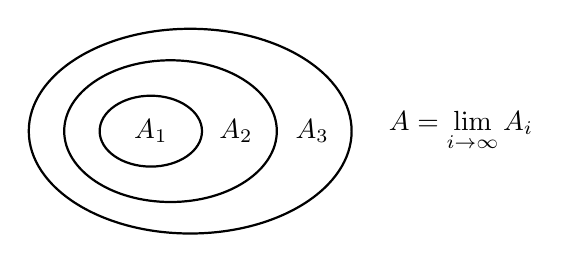
\begin{tikzpicture}
        \draw[thick] (0,0) ellipse (0.65cm and 0.45cm);
        \draw[thick] (0.25,0) ellipse (1.35cm and 0.9cm);
        \draw[thick] (0.5,0) ellipse (2.05cm and 1.3cm);
        \node at (0,0) {$A_1$};
        \node at (1.08,0) {$A_2$};
        \node at (2.05,0) {$A_3$};
        \node[right] at (2.9,0)
            {$A=\lim\limits_{i\to\infty}A_i$};
    \end{tikzpicture}
\end{center}

\begin{definition}[3. Непрерывность сверху]
    Мера $\Pr$ называется \textbf{непрерывной сверху}, если
    для любой невозрастающей последовательности
    $B_i\in\mathcal{F}$, $B_i\supset B_{i+1}$,
    \[
        B=\bigcap_{i=1}^{\infty}B_i
        \quad\Longrightarrow\quad
        \Pr(B)=\lim_{i\to\infty}\Pr(B_i).
    \]
\end{definition}

\begin{theorem}
    Для вероятностной меры на $\sigma$-алгебре условия
    1, 2 и 3 эквивалентны:
    \[
        \text{$\sigma$-аддитивность}
        \quad\Longleftrightarrow\quad
        \text{непрерывность снизу}
        \quad\Longleftrightarrow\quad
        \text{непрерывность сверху}.
    \]
\end{theorem}

\begin{Proof}[$1\implies3$]
    Пусть $B_i\supset B_{i+1}$. Положим
    \[
        A_i=B_i\setminus B_{i+1},
        \qquad B=\bigcap_{i=1}^{\infty}B_i.
    \]
    \begin{center}
        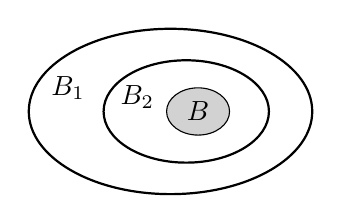
\begin{tikzpicture}
            \draw[thick] (0,0) ellipse (1.8cm and 1.05cm);
            \draw[thick] (0.2,0) ellipse (1.05cm and 0.65cm);
            \fill[gray!35] (0.35,0) ellipse (0.4cm and 0.3cm);
            \draw (0.35,0) ellipse (0.4cm and 0.3cm);
            \node at (-1.3,0.3) {$B_1$};
            \node at (-0.42,0.18) {$B_2$};
            \node at (0.35,0) {$B$};
        \end{tikzpicture}
    \end{center}
    Имеем
    \[
        \left(\bigsqcup_{i=1}^{\infty}A_i\right)\sqcup B=B_1.
    \]
    По $\sigma$-аддитивности
    \[
        \sum_{i=1}^{\infty}\Pr(A_i)+\Pr(B)=\Pr(B_1),
        \qquad \Pr(A_i)=\Pr(B_i)-\Pr(B_{i+1}).
    \]
    Следовательно,
    \[
        \lim_{n\to\infty}
        \underbrace{\sum_{i=1}^{n}
        \bigl(\Pr(B_i)-\Pr(B_{i+1})\bigr)}
        _{\Pr(B_1)-\Pr(B_{n+1})}
        +\Pr(B)=\Pr(B_1).
    \]
    Значит,
    \[
        \Pr(B_1)-\lim_{n\to\infty}\Pr(B_{n+1})
        +\Pr(B)=\Pr(B_1),
    \]
    откуда $\Pr(B)=\lim_{n\to\infty}\Pr(B_{n+1})$.
\end{Proof}


\Needspace{22\baselineskip}
\subsection{Продолжение меры с полукольца на кольцо}

Пусть $m\colon S\to[0;+\infty)$ --- мера на полукольце $S$.
Кольцо $R(S)$ состоит из конечных попарно непересекающихся
объединений элементов $S$:
\[
    R(S)=\left\{\bigsqcup_{i=1}^{n}A_i\colon
        n\in\N,\ A_i\in S\right\}.
\]

\begin{theorem}
    Для $B\in R(S)$ выберем представление
    $B=\bigsqcup_{i=1}^{n}A_i$, где $A_i\in S$, и положим
    \[
        \gamma(B)=\sum_{i=1}^{n}m(A_i).
    \]
    Тогда $\gamma$ определена корректно, является мерой на $R(S)$
    и продолжает $m$:
    \[
        \gamma(B)=m(B)\qquad\forall B\in S.
    \]
\end{theorem}

\begin{Proof}[Независимость от представления]
    Пусть
    \[
        B=\bigsqcup_{i=1}^{n}A_i=\bigsqcup_{j=1}^{k}C_j,
        \qquad A_i,C_j\in S.
    \]
    Положим $D_{ij}=A_i\cap C_j\in S$. Тогда
    \[
        A_i=\bigsqcup_{j=1}^{k}D_{ij},\qquad
        C_j=\bigsqcup_{i=1}^{n}D_{ij}.
    \]
    По конечной аддитивности $m$ имеем
    \[
        \begin{aligned}
            \sum_{i=1}^{n}m(A_i)
            &=\sum_{i=1}^{n}\sum_{j=1}^{k}m(D_{ij})\\
            &=\sum_{j=1}^{k}\sum_{i=1}^{n}m(D_{ij})
              =\sum_{j=1}^{k}m(C_j).
        \end{aligned}
    \]
    Следовательно, значение $\gamma(B)$ не зависит от выбора разбиения.
\end{Proof}

\begin{Proof}[Конечная аддитивность и продолжение исходной меры]
    Неотрицательность $\gamma$ следует из неотрицательности $m$.
    Пусть
    \[
        B=\bigsqcup_{k=1}^{r}B_k,\qquad B_k\in R(S).
    \]
    Представим каждое $B_k$ в виде
    \[
        B_k=\bigsqcup_{j=1}^{n_k}E_{kj},\qquad E_{kj}\in S.
    \]
    Все множества $E_{kj}$ попарно не пересекаются, поэтому
    \[
        \gamma(B)=\sum_{k=1}^{r}\sum_{j=1}^{n_k}m(E_{kj})
                 =\sum_{k=1}^{r}\gamma(B_k).
    \]
    Если $B\in S$, можно выбрать представление из одного множества;
    тогда $\gamma(B)=m(B)$.
\end{Proof}
\endgroup

    \clearpage
\begingroup
\tcbset{myboxstyle/.append style={breakable=false}}
\everymath{\textstyle}
\subsection{Субаддитивность и супераддитивность}

Пусть $\mathcal X$ --- система подмножеств некоторого множества,
а $m\colon\mathcal X\to[0;+\infty)$ --- неотрицательная функция.

\begin{definition}[Субаддитивность]
    Функция $m$ называется \textbf{субаддитивной}, если для любых
    $A,A_1,\ldots,A_n\in\mathcal X$
    \[
        A\subseteq\bigcup_{i=1}^{n}A_i
        \quad\Longrightarrow\quad
        m(A)\leq\sum_{i=1}^{n}m(A_i).
    \]
\end{definition}

\begin{definition}[Супераддитивность]
    Функция $m$ называется \textbf{супераддитивной}, если для любых
    $B,B_1,\ldots,B_r\in\mathcal X$, где $B_j$ попарно не пересекаются,
    \[
        \bigsqcup_{j=1}^{r}B_j\subseteq B
        \quad\Longrightarrow\quad
        \sum_{j=1}^{r}m(B_j)\leq m(B).
    \]
\end{definition}

\begin{theorem}
    Любая мера на полукольце $S$ субаддитивна и супераддитивна.
\end{theorem}

\begin{Proof}[Субаддитивность]
    Пусть $A\subseteq\bigcup_{i=1}^{n}A_i$, где $A,A_i\in S$.
    По лемме о замельчении существует конечное семейство попарно
    непересекающихся множеств $C_j\in S$, для которого
    \[
        A=\bigsqcup_{j\in I}C_j,\qquad
        A_i=\bigsqcup_{j\in I_i}C_j.
    \]
    Каждое $C_j$, входящее в разбиение $A$, входит хотя бы в одно разбиение
    $A_i$. Поэтому по конечной аддитивности и неотрицательности
    \[
        m(A)=\sum_{j\in I}m(C_j)
        \leq\sum_{i=1}^{n}\sum_{j\in I_i}m(C_j)
        =\sum_{i=1}^{n}m(A_i).
    \]
\end{Proof}

\begin{Proof}[Супераддитивность]
    По свойствам полукольца найдутся попарно непересекающиеся $D_k\in S$:
    \[
        B\setminus\bigsqcup_{j=1}^{r}B_j
        =\bigsqcup_{k=1}^{\ell}D_k,\qquad D_k\in S.
    \]
    По аддитивности $m(B)=\sum_{j=1}^{r}m(B_j)+\sum_{k=1}^{\ell}m(D_k)
    \geq\sum_{j=1}^{r}m(B_j)$.
\end{Proof}

\newpage
\begin{theorem}[Обратное утверждение]
    Если неотрицательная функция $m$ на полукольце $S$ субаддитивна
    и супераддитивна, то она конечно аддитивна, то есть является мерой.
\end{theorem}

\begin{Proof}
    При $A=\bigsqcup_{i=1}^{n}A_i$, $A,A_i\in S$, два свойства дают
    \[
        m(A)\leq\sum_{i=1}^{n}m(A_i)\leq m(A).
    \]
    Следовательно, обе оценки обращаются в равенство.
\end{Proof}

\subsection{Счётные аналоги}

\begin{definition}[$\sigma$-субаддитивность]
    Функция $m$ называется \textbf{$\sigma$-субаддитивной}, если для любых
    $A,A_1,A_2,\ldots\in\mathcal X$
    \[
        A\subseteq\bigcup_{i=1}^{\infty}A_i
        \quad\Longrightarrow\quad
        m(A)\leq\sum_{i=1}^{\infty}m(A_i).
    \]
\end{definition}

\begin{definition}[$\sigma$-супераддитивность]
    Функция $m$ называется \textbf{$\sigma$-супераддитивной}, если для любых
    $B,B_1,B_2,\ldots\in\mathcal X$, где $B_j$ попарно не пересекаются,
    \[
        \bigsqcup_{j=1}^{\infty}B_j\subseteq B
        \quad\Longrightarrow\quad
        \sum_{j=1}^{\infty}m(B_j)\leq m(B).
    \]
\end{definition}

\begin{theorem}
    Любая мера на полукольце $S$ является $\sigma$-супераддитивной.
\end{theorem}

\begin{Proof}
    Если $\bigsqcup_{j=1}^{\infty}B_j\subseteq B$, то для каждого $n\in\N$
    \[
        \bigsqcup_{j=1}^{n}B_j\subseteq B,
        \qquad\sum_{j=1}^{n}m(B_j)\leq m(B).
    \]
    Переходя к пределу при $n\to\infty$, получаем требуемое неравенство.
\end{Proof}

\newpage
\subsection{Критерий счётной аддитивности}

\begin{theorem}
    Мера $m$ на полукольце $S$ является $\sigma$-аддитивной
    тогда и только тогда, когда она $\sigma$-субаддитивна.
\end{theorem}

\begin{Proof}[Достаточность]
    Пусть $m$ является $\sigma$-субаддитивной. Если
    $A=\bigsqcup_{i=1}^{\infty}A_i$, где $A,A_i\in S$, то
    по $\sigma$-субаддитивности и $\sigma$-супераддитивности
    \[
        m(A)\leq\sum_{i=1}^{\infty}m(A_i)\leq m(A).
    \]
    Значит, $m(A)=\sum_{i=1}^{\infty}m(A_i)$.
\end{Proof}

\begin{Proof}[Необходимость]
    Пусть $m$ является $\sigma$-аддитивной и
    $A\subseteq\bigcup_{i=1}^{\infty}A_i$, где $A,A_i\in S$.
    Положим $A_i'=A\cap A_i\in S$. Тогда
    \[
        A=\bigcup_{i=1}^{\infty}A_i',\qquad m(A_i')\leq m(A_i).
    \]
    Исключим из каждого множества уже учтённые части. Для $i\geq2$
    представим
    \[
        A_i'\setminus\bigcup_{k=1}^{i-1}A_k'
        =\bigsqcup_{j=1}^{r_i}B_{ij},\qquad B_{ij}\in S.
    \]
    Все полученные множества попарно не пересекаются, и
    \[
        A=A_1'\sqcup\bigsqcup_{i=2}^{\infty}
                       \bigsqcup_{j=1}^{r_i}B_{ij}.
    \]
    По конечной супераддитивности
    $\sum_{j=1}^{r_i}m(B_{ij})\leq m(A_i')$.
    Поэтому по $\sigma$-аддитивности
    \[
        \begin{aligned}
            m(A)
            &=m(A_1')+\sum_{i=2}^{\infty}\sum_{j=1}^{r_i}m(B_{ij})\\
            &\leq\sum_{i=1}^{\infty}m(A_i')
             \leq\sum_{i=1}^{\infty}m(A_i).
        \end{aligned}
    \]
\end{Proof}

\newpage
\subsection{Счётная аддитивность меры Лебега--Стилтьеса}

Пусть $S$ --- полукольцо промежутков, введённое ранее, а
$F\colon\R\to\R$ ограничена, не убывает и непрерывна справа.
Мера $m$ задаётся равенством $m((a;b])=F(b)-F(a)$
с соответствующими предельными формулами для неограниченных промежутков.

\begin{theorem}
    Мера Лебега--Стилтьеса $m$ на полукольце $S$ является
    $\sigma$-аддитивной.
\end{theorem}

\begin{Proof}[Счётная субаддитивность на ограниченном промежутке]
    По доказанному критерию достаточно проверить $\sigma$-субаддитивность.
    Пусть
    \[
        (a;b]\subseteq\bigcup_{i=1}^{\infty}(a_i;b_i].
    \]
    Зафиксируем $\eps>0$. По непрерывности $F$ справа выберем
    $a'\in(a;b)$ и $b_i'>b_i$ так, чтобы
    \[
        F(a')-F(a)<\frac\eps2,\qquad
        F(b_i')-F(b_i)<\frac{\eps}{2^{i+1}}.
    \]
    Открытые интервалы $(a_i;b_i')$ покрывают отрезок $[a';b]$.
    По лемме Гейне--Бореля существует конечное подпокрытие
    с множеством индексов $I\subset\N$:
    \[
        [a';b]\subseteq\bigcup_{i\in I}(a_i;b_i').
    \]
    Следовательно, $(a';b]\subseteq\bigcup_{i\in I}(a_i;b_i']$.
    По конечной субаддитивности
    \[
        \begin{aligned}
            F(b)-F(a')
            &\leq\sum_{i\in I}\bigl(F(b_i')-F(a_i)\bigr)\\
            &\leq\sum_{i=1}^{\infty}
                 \left(F(b_i)-F(a_i)+\frac{\eps}{2^{i+1}}\right)\\
            &=\sum_{i=1}^{\infty}m((a_i;b_i])+\frac\eps2.
        \end{aligned}
    \]
    Прибавляя $F(a')-F(a)<\eps/2$, получаем
    \[
        m((a;b])\leq\sum_{i=1}^{\infty}m((a_i;b_i])+\eps.
    \]
    Устремляя $\eps$ к нулю, получаем требуемое неравенство.
\end{Proof}

\begin{remark}[Неограниченные промежутки]
    Для покрытия лучами используется то же рассуждение с открытыми лучами.
    Если покрываемый промежуток неограничен, сначала рассматривают его
    пересечение с $(-M;M]$, затем переходят к пределу при $M\to\infty$
    по формулам через $F(-\infty)$ и $F(+\infty)$.
\end{remark}
\endgroup

    \clearpage
\begingroup
\tcbset{myboxstyle/.append style={breakable=false}}
\everymath{\textstyle}
\subsection{Счётная аддитивность продолжения меры}

Пусть $S$ --- полуалгебра подмножеств $\Omega$, то есть полукольцо,
содержащее $\Omega$, а $m$ --- конечная $\sigma$-аддитивная мера на $S$.
Обозначим через $\gamma$ её продолжение на $R(S)$:
\[
    \gamma\left(\bigsqcup_{i=1}^{n}A_i\right)
    =\sum_{i=1}^{n}m(A_i),\qquad A_i\in S.
\]
Поскольку $\Omega\in S$, кольцо $R(S)$ является алгеброй.

\begin{theorem}
    Продолжение $\gamma$ является $\sigma$-аддитивной мерой на $R(S)$.
    В частности, оно $\sigma$-субаддитивно.
\end{theorem}

\subsection{Внешняя мера Лебега}

\begin{definition}
    Для любого $A\subseteq\Omega$ положим
    \[
        \mu^*(A)=\inf\left\{
            \sum_{i=1}^{\infty}m(A_i):\
            A\subseteq\bigcup_{i=1}^{\infty}A_i,\quad A_i\in S
        \right\}.
    \]
    Функция $\mu^*\colon2^\Omega\to[0;+\infty)$ называется
    \textbf{внешней мерой Лебега}, порождённой $m$.
    Инфимум берётся по всем счётным покрытиям $A$ элементами $S$.
\end{definition}

\begin{remark}[Конечность внешней меры]
    Любое $A\subseteq\Omega$ покрывается множеством $\Omega\in S$, поэтому
    \[
        0\leq\mu^*(A)\leq m(\Omega)<\infty.
    \]
    Конечное покрытие можно дополнить пустыми множествами.
    В частности, $\mu^*(\varnothing)=0$.
\end{remark}

\begin{theorem}[Совпадение с мерой на алгебре]
    Для любого $A\in R(S)$ справедливо равенство $\mu^*(A)=\gamma(A)$.
\end{theorem}

\begin{Proof}
    Пусть $A=\bigsqcup_{i=1}^{n}A_i$, $A_i\in S$.
    Это покрытие $A$, поэтому
    \[
        \mu^*(A)\leq\sum_{i=1}^{n}m(A_i)=\gamma(A).
    \]
    С другой стороны, для любого покрытия $A\subseteq\bigcup_{j=1}^{\infty}B_j$,
    $B_j\in S$, по $\sigma$-субаддитивности $\gamma$
    \[
        \gamma(A)\leq\sum_{j=1}^{\infty}\gamma(B_j)
        =\sum_{j=1}^{\infty}m(B_j).
    \]
    Переходя к инфимуму по покрытиям, получаем $\gamma(A)\leq\mu^*(A)$.
\end{Proof}

\newpage
\subsection{Свойства внешней меры}

\begin{example}[Внешняя мера не обязана быть аддитивной]
    Пусть
    \[
        \Omega=\{1,2,3\},\qquad
        S=\{\varnothing,\{1,2\},\{3\},\Omega\},
    \]
    а мера на $S$ задана значениями
    \[
        m(\varnothing)=0,\quad m(\{1,2\})=2,\quad
        m(\{3\})=0,\quad m(\Omega)=2.
    \]
    Тогда $\mu^*(\{1\})=\mu^*(\{2\})=2$ и $\mu^*(\{1,2\})=2$.
    Следовательно,
    \[
        \mu^*(\{1\}\sqcup\{2\})=2
        \ne\mu^*(\{1\})+\mu^*(\{2\})=4.
    \]
\end{example}

\begin{theorem}[Счётная субаддитивность]
    Для любых $A,A_1,A_2,\ldots\subseteq\Omega$
    \[
        A\subseteq\bigcup_{i=1}^{\infty}A_i
        \quad\Longrightarrow\quad
        \mu^*(A)\leq\sum_{i=1}^{\infty}\mu^*(A_i).
    \]
\end{theorem}

\begin{Proof}
    Если сумма справа бесконечна, утверждение очевидно.
    Пусть она конечна. Зафиксируем $\eps>0$. По определению инфимума
    для каждого $i$ выберем покрытие
    \[
        A_i\subseteq\bigcup_{j=1}^{\infty}B_{ij},\qquad B_{ij}\in S,
        \qquad
        \sum_{j=1}^{\infty}m(B_{ij})<\mu^*(A_i)+\frac{\eps}{2^i}.
    \]
    Счётное семейство всех $B_{ij}$ покрывает $A$. Поэтому
    \[
        \begin{aligned}
            \mu^*(A)
            &\leq\sum_{i=1}^{\infty}\sum_{j=1}^{\infty}m(B_{ij})\\
            &\leq\sum_{i=1}^{\infty}\mu^*(A_i)
                 +\sum_{i=1}^{\infty}\frac{\eps}{2^i}
             =\sum_{i=1}^{\infty}\mu^*(A_i)+\eps.
        \end{aligned}
    \]
    Устремляя $\eps$ к нулю, получаем требуемое неравенство.
\end{Proof}

\newpage
\begin{theorem}[Оценка через симметрическую разность]
    Для любых $A,B\subseteq\Omega$
    \[
        |\mu^*(A)-\mu^*(B)|\leq\mu^*(A\mathbin{\triangle}B).
    \]
\end{theorem}

\begin{Proof}
    Из включений
    \[
        A\subseteq B\cup(A\mathbin{\triangle}B),\qquad
        B\subseteq A\cup(A\mathbin{\triangle}B)
    \]
    и субаддитивности следует
    \[
        \begin{aligned}
            \mu^*(A)&\leq\mu^*(B)+\mu^*(A\mathbin{\triangle}B),\\
            \mu^*(B)&\leq\mu^*(A)+\mu^*(A\mathbin{\triangle}B).
        \end{aligned}
    \]
    Все величины конечны, поэтому эти два неравенства дают требуемую оценку.
\end{Proof}

\subsection{Измеримые по Лебегу множества}

\begin{definition}
    Множество $A\subseteq\Omega$ называется \textbf{измеримым по Лебегу}
    относительно построенной внешней меры, если
    \[
        \forall\eps>0\quad\exists A_\eps\in R(S):\quad
        \mu^*(A\mathbin{\triangle}A_\eps)<\eps.
    \]
    Обозначим систему всех таких множеств через $M$.
\end{definition}

\begin{theorem}
    $R(S)\subseteq M$.
\end{theorem}

\begin{Proof}
    Для $A\in R(S)$ и любого $\eps>0$ выберем $A_\eps=A$.
    Тогда $\mu^*(A\mathbin{\triangle}A_\eps)=\mu^*(\varnothing)=0<\eps$.
\end{Proof}

\begin{theorem}
    Система $M$ измеримых по Лебегу множеств является алгеброй.
\end{theorem}

\newpage
\begin{Proof}[Замкнутость относительно пересечения]
    Пусть $A,B\in M$ и $\eps>0$. Выберем
    $A_{\eps/2},B_{\eps/2}\in R(S)$ так, чтобы
    \[
        \mu^*(A\mathbin{\triangle}A_{\eps/2})<\frac\eps2,
        \qquad
        \mu^*(B\mathbin{\triangle}B_{\eps/2})<\frac\eps2.
    \]
    Тогда $A_{\eps/2}\cap B_{\eps/2}\in R(S)$ и
    \[
        (A\cap B)\mathbin{\triangle}(A_{\eps/2}\cap B_{\eps/2})
        \subseteq
        (A\mathbin{\triangle}A_{\eps/2})
        \cup(B\mathbin{\triangle}B_{\eps/2}).
    \]
    По субаддитивности
    \[
        \begin{aligned}
            &\mu^*\bigl((A\cap B)\mathbin{\triangle}
                           (A_{\eps/2}\cap B_{\eps/2})\bigr)\\
            &\qquad\leq\mu^*(A\mathbin{\triangle}A_{\eps/2})
                      +\mu^*(B\mathbin{\triangle}B_{\eps/2})<\eps.
        \end{aligned}
    \]
    Следовательно, $A\cap B\in M$.
\end{Proof}

\begin{Proof}[Замкнутость относительно симметрической разности]
    Для тех же приближений
    $A_{\eps/2}\mathbin{\triangle}B_{\eps/2}\in R(S)$ и
    \[
        \begin{aligned}
            &(A\mathbin{\triangle}B)\mathbin{\triangle}
                (A_{\eps/2}\mathbin{\triangle}B_{\eps/2})\\
            &\qquad\subseteq
                (A\mathbin{\triangle}A_{\eps/2})
                \cup(B\mathbin{\triangle}B_{\eps/2}).
        \end{aligned}
    \]
    Поэтому
    \[
        \begin{aligned}
            &\mu^*\bigl((A\mathbin{\triangle}B)\mathbin{\triangle}
                (A_{\eps/2}\mathbin{\triangle}B_{\eps/2})\bigr)\\
            &\qquad\leq\mu^*(A\mathbin{\triangle}A_{\eps/2})
                      +\mu^*(B\mathbin{\triangle}B_{\eps/2})<\eps.
        \end{aligned}
    \]
    Следовательно, $A\mathbin{\triangle}B\in M$.
    Замкнутость относительно пересечения и симметрической разности
    означает, что $M$ --- кольцо. Так как $\Omega\in R(S)\subseteq M$,
    это кольцо является алгеброй.
\end{Proof}
\endgroup

    \clearpage
\begingroup
\tcbset{myboxstyle/.append style={breakable=false}}
\section{Математическое ожидание и дисперсия}

\subsection{Математическое ожидание}

Пусть $(\Omega,\mathcal F,\Pr)$ --- вероятностное пространство,
а $\xi\colon\Omega\to\R$ --- случайная величина.
Её распределение задаётся вероятностной мерой
\[
    \Pr_\xi(B)=\Pr\{\xi\in B\},\qquad B\in\mathcal B(\R).
\]

\subsubsection{Конечная модель и среднее арифметическое}

Пусть $\Omega=\{\omega_1,\ldots,\omega_n\}$. Проведём $N$ опытов
с результатами $\omega^1,\ldots,\omega^N$ и обозначим через $N_i$
число появлений исхода $\omega_i$. Тогда среднее наблюдаемых значений равно
\[
    \frac1N\sum_{j=1}^{N}\xi(\omega^j)
    =\sum_{i=1}^{n}\xi(\omega_i)\frac{N_i}{N}.
\]
В вероятностной модели частотам $N_i/N$ соответствуют вероятности
$\Pr\{\omega_i\}$.

\begin{definition}[Математическое ожидание в конечной модели]
    \textbf{Математическим ожиданием} случайной величины $\xi$ называется
    \[
        \EE\xi=\sum_{i=1}^{n}\xi(\omega_i)\Pr\{\omega_i\}.
    \]
    Используется также обозначение $M\xi$.
\end{definition}

\begin{definition}[Общее определение]
    Математическое ожидание случайной величины $\xi$ --- интеграл Лебега
    \[
        \EE\xi=\int_\Omega\xi(\omega)\,\diff\Pr(\omega).
    \]
    Конечное математическое ожидание существует при условии
    \[
        \int_\Omega|\xi(\omega)|\,\diff\Pr(\omega)<\infty.
    \]
\end{definition}

\begin{theorem}[Вычисление по распределению]
    Если в конечной модели $\xi$ принимает различные значения
    $x_1,\ldots,x_k$ с вероятностями $p_i=\Pr\{\xi=x_i\}$, то
    \[
        \EE\xi=\sum_{i=1}^{k}x_i p_i.
    \]
\end{theorem}

\begin{Proof}
    Сгруппируем исходы, на которых $\xi$ принимает одинаковое значение:
    \[
        \sum_{\omega\in\Omega}\xi(\omega)\Pr\{\omega\}
        =\sum_{i=1}^{k}x_i
          \sum_{\omega:\,\xi(\omega)=x_i}\Pr\{\omega\}
        =\sum_{i=1}^{k}x_i p_i.
    \]
\end{Proof}

\newpage
\subsubsection{Дискретное и абсолютно непрерывное распределения}

\begin{definition}[Дискретное распределение]
    Для распределения $\{(x_i,p_i)\}_i$ математическое ожидание равно
    \[
        \EE\xi=\sum_i x_i p_i,
        \qquad\text{если}\quad \sum_i |x_i|p_i<\infty.
    \]
    Таким образом, требуется абсолютная сходимость ряда.
\end{definition}

\begin{example}[Распределение Пуассона]
    Если $\xi\sim\operatorname{Poiss}(\lambda)$, $\lambda>0$, то
    \[
        \Pr\{\xi=k\}=e^{-\lambda}\frac{\lambda^k}{k!},
        \qquad k=0,1,2,\ldots
    \]
    Все слагаемые неотрицательны, и
    \[
        \begin{aligned}
            \EE\xi
            &=\sum_{k=0}^{\infty}k e^{-\lambda}\frac{\lambda^k}{k!}
             =\lambda e^{-\lambda}
                \sum_{k=1}^{\infty}\frac{\lambda^{k-1}}{(k-1)!}\\
            &=\lambda e^{-\lambda}
                \sum_{m=0}^{\infty}\frac{\lambda^m}{m!}
             =\lambda e^{-\lambda}e^\lambda=\lambda.
        \end{aligned}
    \]
\end{example}

\begin{definition}[Абсолютно непрерывное распределение]
    Если $\xi$ имеет плотность $p_\xi$, то
    \[
        \EE\xi=\int_{-\infty}^{+\infty}x p_\xi(x)\,\diff x,
        \qquad\text{если}\quad
        \int_{-\infty}^{+\infty}|x|p_\xi(x)\,\diff x<\infty.
    \]
    Если интеграл записан как несобственный интеграл Римана,
    требуется его абсолютная сходимость.
\end{definition}

Для малого промежутка $\Delta_i$ около точки $x_i$, в которой плотность
непрерывна,
\[
    \Pr\{\xi\in\Delta_i\}\approx p_\xi(x_i)|\Delta_i|.
\]
Поэтому суммам $\sum_i x_i\Pr\{\xi\in\Delta_i\}$ соответствуют
интегральные суммы $\sum_i x_i p_\xi(x_i)|\Delta_i|$.

\begin{consequence}
    Математическое ожидание определяется распределением случайной величины:
    \[
        \EE\xi=\int_\R x\,\diff\Pr_\xi(x).
    \]
\end{consequence}

\newpage
\subsection{Свойства математического ожидания}

\begin{theorem}[Ожидание константы и линейность]
    Для $c\in\R$ имеем $\EE c=c$.
    Если существуют конечные $\EE\xi_1$ и $\EE\xi_2$, то для любых
    $a_1,a_2\in\R$ существует математическое ожидание их линейной комбинации и
    \[
        \EE(a_1\xi_1+a_2\xi_2)
        =a_1\EE\xi_1+a_2\EE\xi_2.
    \]
\end{theorem}

\begin{Proof}[Линейность в дискретном случае]
    Пусть $\xi_1$ принимает значения $x_i$, а $\xi_2$ --- значения $y_j$.
    Обозначим
    \[
        p_{ij}=\Pr\{\xi_1=x_i,\ \xi_2=y_j\},\qquad
        p_i=\Pr\{\xi_1=x_i\},\quad q_j=\Pr\{\xi_2=y_j\}.
    \]
    По счётной аддитивности вероятности
    \[
        \sum_j p_{ij}=p_i,\qquad \sum_i p_{ij}=q_j.
    \]
    Сначала проверим абсолютную сходимость:
    \[
        \begin{aligned}
            \sum_{i,j}|a_1x_i+a_2y_j|p_{ij}
            &\leq |a_1|\sum_i|x_i|\sum_jp_{ij}
                  +|a_2|\sum_j|y_j|\sum_ip_{ij}\\
            &=|a_1|\sum_i|x_i|p_i+|a_2|\sum_j|y_j|q_j<\infty.
        \end{aligned}
    \]
    Следовательно, суммы можно перегруппировать:
    \[
        \begin{aligned}
            \EE(a_1\xi_1+a_2\xi_2)
            &=\sum_{i,j}(a_1x_i+a_2y_j)p_{ij}\\
            &=a_1\sum_i x_i p_i+a_2\sum_j y_j q_j\\
            &=a_1\EE\xi_1+a_2\EE\xi_2.
        \end{aligned}
    \]
\end{Proof}

\begin{theorem}[Монотонность]
    Если $\xi\geq\eta$ почти наверное и оба математических ожидания конечны,
    то $\EE\xi\geq\EE\eta$.
\end{theorem}

\begin{Proof}
    Для $\zeta=\xi-\eta\geq0$ имеем $\EE\zeta\geq0$.
    По линейности $\EE\zeta=\EE\xi-\EE\eta$, откуда
    $\EE\xi\geq\EE\eta$.
\end{Proof}

\newpage
\begin{theorem}[Оценка модуля ожидания]
    Если $\EE\xi$ конечно, то
    \[
        |\EE\xi|\leq\EE|\xi|.
    \]
\end{theorem}

\begin{Proof}
    Ожидание $\EE|\xi|$ конечно по условию абсолютной интегрируемости.
    Из $-|\xi|\leq\xi\leq|\xi|$, монотонности и линейности следует
    \[
        -\EE|\xi|\leq\EE\xi\leq\EE|\xi|.
    \]
\end{Proof}

\subsection{Дисперсия}

\begin{example}[Одинаковое ожидание и различный разброс]
    Пусть
    \[
        \Pr\{\xi_1=-1\}=\Pr\{\xi_1=1\}=\frac12,\qquad
        \Pr\{\xi_2=-100\}=\Pr\{\xi_2=100\}=\frac12.
    \]
    Тогда $\EE\xi_1=\EE\xi_2=0$, но значения второй величины
    дальше от математического ожидания.
\end{example}

\begin{definition}
    \textbf{Дисперсией} случайной величины $\xi$ с конечным математическим
    ожиданием называется
    \[
        \DD\xi=\operatorname{Var}\xi
        =\EE(\xi-\EE\xi)^2.
    \]
    Конечная дисперсия существует, если $\EE\xi^2<\infty$.
\end{definition}

\begin{theorem}[Формула для вычисления дисперсии]
    При $\EE\xi^2<\infty$ справедливо равенство
    \[
        \DD\xi=\EE\xi^2-(\EE\xi)^2.
    \]
\end{theorem}

\begin{Proof}
    По линейности математического ожидания
    \[
        \begin{aligned}
            \DD\xi
            &=\EE\bigl(\xi^2-2\xi\EE\xi+(\EE\xi)^2\bigr)\\
            &=\EE\xi^2-2(\EE\xi)^2+(\EE\xi)^2\\
            &=\EE\xi^2-(\EE\xi)^2.
        \end{aligned}
    \]
\end{Proof}
\endgroup

    \clearpage
\begingroup
\tcbset{myboxstyle/.append style={breakable=false}}
\everymath{\textstyle}
\subsection{Математическое ожидание функции случайных величин}

Пусть $f\colon\R^2\to\R$ --- борелевская функция.

\begin{theorem}[Дискретное совместное распределение]
    Если $p_{ij}=\Pr\{\xi=x_i,\eta=y_j\}$ и
    $\sum_{i,j}|f(x_i,y_j)|p_{ij}<\infty$, то
    \[
        \EE f(\xi,\eta)=\sum_{i,j}f(x_i,y_j)p_{ij}.
    \]
\end{theorem}

\begin{theorem}[Абсолютно непрерывное совместное распределение]
    Если $(\xi,\eta)$ имеет плотность $p_{\xi,\eta}$ и
    \[
        \iint_{\R^2}|f(x,y)|p_{\xi,\eta}(x,y)\,\diff x\,\diff y<\infty,
    \]
    то
    \[
        \EE f(\xi,\eta)
        =\iint_{\R^2}f(x,y)p_{\xi,\eta}(x,y)\,\diff x\,\diff y.
    \]
\end{theorem}

\subsection{Ковариация}

\begin{definition}
    Для случайных величин $\xi$ и $\eta$ с конечными вторыми моментами
    \textbf{ковариацией} называется число
    \[
        \operatorname{cov}(\xi,\eta)
        =\EE\bigl[(\xi-\EE\xi)(\eta-\EE\eta)\bigr].
    \]
\end{definition}

\begin{theorem}[Свойства ковариации]
    При конечности вторых моментов справедливы следующие свойства.
    \begin{enumerate}
        \item $\operatorname{cov}(\xi,\xi)=\DD\xi$.
        % Дополнение из лекции 17, с. 5.
        \item $\operatorname{cov}(\xi,\eta)=\EE(\xi\eta)-\EE\xi\cdot\EE\eta$.
        \item Ковариация является билинейной формой: для $a,b\in\R$
        \[
            \begin{aligned}
                \operatorname{cov}(a\xi+b\eta,\zeta)
                &=a\operatorname{cov}(\xi,\zeta)+b\operatorname{cov}(\eta,\zeta),\\
                \operatorname{cov}(\zeta,a\xi+b\eta)
                &=a\operatorname{cov}(\zeta,\xi)+b\operatorname{cov}(\zeta,\eta).
            \end{aligned}
        \]
        \item Из независимости $\xi$ и $\eta$ следует
        $\operatorname{cov}(\xi,\eta)=0$. Обратное утверждение неверно.
    \end{enumerate}
\end{theorem}
% Дополнение из лекции 17, с. 5.
\begin{theorem}[Дисперсия суммы]
    Если $\xi$ и $\eta$ имеют конечные вторые моменты, то
    \[
        \DD(\xi+\eta)=\DD\xi+2\operatorname{cov}(\xi,\eta)+\DD\eta.
    \]
    В частности, для независимых $\xi$ и $\eta$
    \[
        \DD(\xi+\eta)=\DD\xi+\DD\eta.
    \]
\end{theorem}

\begin{Proof}
    По линейности математического ожидания
    \[
        \begin{aligned}
            \DD(\xi+\eta)
            &=\EE\bigl[(\xi-\EE\xi)+(\eta-\EE\eta)\bigr]^2\\
            &=\EE(\xi-\EE\xi)^2
              +2\EE\bigl[(\xi-\EE\xi)(\eta-\EE\eta)\bigr]
              +\EE(\eta-\EE\eta)^2\\
            &=\DD\xi+2\operatorname{cov}(\xi,\eta)+\DD\eta.
        \end{aligned}
    \]
    При независимости ковариация равна нулю.
\end{Proof}
\endgroup

    % \input{./lectures/lectures_03_[18.09.2026].tex}
    % \input{./lectures/lectures_04_[25.09.2026].tex}
    
    %\section{Информация о курсе} 
\subsection{Оценка} 

Формула итоговой оценки за курс:
\[ 
\begin{aligned}
\text{О} ={} & 0.15 \cdot \text{ДЗ} + 0.1 \cdot \text{Quiz} + 0.15 \cdot \text{Контест} + {} \\
& 0.2 \cdot \text{КР (БЛОК)} + 0.25 \cdot \text{Коллок (БЛОК)} + {} \\
& 0.05 \cdot \text{Бонус от семинариста} + 0.2 \cdot \text{Коллок по доп.\ материалу} 
\end{aligned}
\]

\section{Введение}

\begin{definition}[Случайный эксперимент]
    \textbf{Случайный эксперимент} --- это процесс, наблюдение или действие, результат которого невозможно точно предсказать заранее (до его проведения). 
    
    Чтобы эксперимент можно было изучать методами теории вероятностей, он должен обладать следующими свойствами:
    \begin{itemize}
        \item \textbf{Отсутствие детерминированной регулярности:} при многократном повторении эксперимента в неизменных условиях результаты могут различаться (исход единичного опыта случаен).
        \item \textbf{Воспроизводимость эксперимента:} эксперимент теоретически или практически можно повторить бесконечное число раз в одних и тех же контролируемых условиях. Его проведение и исход не должны быть завязаны на уникальные свойства или волю конкретной личности.
        \item \textbf{Статистическая устойчивость:} при очень большом числе повторений частота появления того или иного исхода стабилизируется и стремится к фиксированному числу (вероятности).
        \[
        \frac{N_{1, N}}{N_1} \approx \frac{N_{2, N}}{N_2} \approx \ldots \approx \frac{N_{k, N}}{N_k}
        \]
    \end{itemize}
\end{definition}

Сопоставим каждому результату эксперимента свою $\omega$ --- \textbf{элементарный исход}. Множество всех элементарных исходов обозначается как $\Omega$:
\[
    \Omega = \{\omega\} 
\]

\begin{example}[Пример: Бросок двух игральных костей]
    Кидаются 2 кости, нас интересует сумма. Варианты выбора пространства $\Omega$:
    \begin{enumerate}[label=\arabic*)]
        \item $\omega \in \{2, \dots, 12\}, \quad |\Omega| = 11$
        \item $\omega = (i_1, i_2), \quad i_j \in \{1, \dots, 6\}, \quad |\Omega| = 36$
        \item $\omega = \{i_1, i_2\}, \quad |\Omega| = \frac{36-6}{2} + 6 = 21$
    \end{enumerate}
\end{example}

\subsection{События}

\begin{definition}[Случайное событие]
    \textbf{Случайное событие} --- это подмножество пространства элементарных исходов: $\mathcal{A} \subset \Omega$.
\end{definition}

\begin{definition}[Вероятность]
    \textbf{Вероятность} события $\mathcal{A}$ --- это предел относительной частоты его появления при стремлении числа экспериментов к бесконечности:
    \[
        \frac{N_{\mathcal{A}}}{N} \xrightarrow[N \to \infty]{} \Pr(\mathcal{A})
    \]
\end{definition}

\subsection{Математические модели}

Любая математическая модель в теории вероятностей состоит из трех объектов: $(\Omega, \mathcal{F}, \Pr)$, где: 
\begin{itemize}
    \item $\Omega$ --- пространство элементарных исходов;
    \item $\mathcal{F}$ --- множество событий, такое что $\mathcal{F} \subset 2^{\Omega}$ ($\sigma$-алгебра);
    \item $\Pr$ --- вероятностная мера, задающая функцию $\Pr \colon \mathcal{F} \to [0; 1]$.
\end{itemize}

\begin{exercise}[О выборе $\mathcal{F}$]
    Всегда ли $\mathcal{F} = 2^{\Omega}$? Верно ли, что $\Omega \in \mathcal{F}$?
\end{exercise}

\subsubsection{Свойства вероятностной меры}

\begin{itemize}
    \item Нормированность: $\Pr(\Omega) = 1$.
    \item Вероятность невозможного события: $\Pr(\varnothing) = 0$. 
    \item \textit{(Отсылка к линейности: $\Pr(\varnothing) = 0 \implies f(\alpha \vec{x} + \beta \vec{y}) = \alpha f(\vec{x}) + \beta f(\vec{y})$)}.
    \item \textbf{Аддитивность:} для несовместных событий (т.е. $\mathcal{A} \cap \mathcal{B} = \varnothing$):
    \[
        \Pr(\mathcal{A} \sqcup \mathcal{B}) = \Pr(\mathcal{A}) + \Pr(\mathcal{B}),
    \]
    где $\sqcup$ --- дизъюнктивное объединение.
\end{itemize}

\subsection{Дискретные модели}

Пусть $\Omega$ --- конечное множество. Тогда:
\[
    \mathcal{F} = 2^{\Omega} \implies \forall \omega \in \Omega \colon \{\omega\} \in \mathcal{F}, \quad |\mathcal{F}| = 2^{|\Omega|}
\]

Как задается $\Pr$? Достаточно задать вероятности каждого исхода:
\[
    \forall \omega \in \Omega \colon \Pr(\omega)
\]
Тогда для любого события $\mathcal{A} \in \mathcal{F}$ ($\mathcal{A} \subset \Omega$) вероятность равна сумме вероятностей входящих в него исходов:
\[
    \Pr(\mathcal{A}) = \Sum{\omega \in \mathcal{A}}{} \Pr(\omega)
\]

\subsubsection{Классические дискретные модели}

\begin{definition}[Классическая модель]
    \textbf{Классическая модель} --- это дискретная модель, в которой все исходы равновероятны: $\Pr(\omega) = \text{const}$.
\end{definition}

Найдем эту константу из свойства нормированности:
\[
    1 = \Pr(\Omega) = \Pr\l(\bigsqcup^{|\Omega|}_{i = 1} \{\omega_i\}\r) = \Sum{i = 1}{|\Omega|} \Pr(\omega_i) = |\Omega| \cdot \text{const} \implies \text{const} = \frac{1}{|\Omega|}
\]
Следовательно, вероятность любого события в классической модели:
\[
    \Pr(\mathcal{A}) = \Sum{\omega \in \mathcal{A}}{} \Pr(\omega) = \Sum{\omega \in \mathcal{A}}{} \frac{1}{|\Omega|} = \frac{|\mathcal{A}|}{|\Omega|}
\]

\begin{example}[Пример: Два кубика в классической модели]
    \begin{itemize}
        \item Различимые кубики: $\omega = (i_1, i_2), \quad |\Omega| = 36$.
        \[
            \mathcal{F} = 2^{\Omega}, \quad \Pr(\mathcal{A}) = \frac{|\mathcal{A}|}{36}
        \]
        \item Неразличимые кубики: $\omega = \{i_1, i_2\}, \quad |\Omega| = 21$.
        \[
            \mathcal{F} = 2^{\Omega}, \quad \Pr(\omega) \neq \text{const} \quad \text{(модель перестает быть классической!)}
        \]
    \end{itemize}
\end{example}

\begin{task}[Урновая схема: выбор с возвращением]
    Есть $N$ шариков: $M$ --- красных (1), $N - M$ --- черных (0). 
    Вытаскиваем $n$ шариков с возвращением. Какова вероятность вытащить ровно $k$ красных шариков (в любом порядке)?
\end{task}

\begin{solution}
    Если мы обозначим элементарный исход как: 
    \[
        \omega = (i_1, \dots, i_n), \quad i_j \in \{0, 1\}
    \]
    то исходы перестанут быть равновероятными. 

    Рассмотрим элементарный исход как упорядоченный набор вытащенных шариков:
    \[
        \omega = (i_1, \dots, i_n), \quad i_j \in \{1, \dots, N\}
    \]
    где номера $1, \dots, M$ --- красные, а $M+1, \dots, N$ --- черные шары.
    
    Общее число исходов:
    \[
        |\Omega| = N^n
    \]
    Число благоприятных исходов (выбираем $k$ позиций для красных шаров из $n$ возможных):
    \[
        |\mathcal{A}| = C_n^k \cdot M^k \cdot (N - M)^{n - k}
    \]
    Вероятность события:
    \[
        \Pr(\mathcal{A}) = \frac{|\mathcal{A}|}{|\Omega|} = \frac{C_n^k \cdot M^k \cdot (N - M)^{n-k}}{N^n} = C_n^k \l( \frac{M}{N} \r)^k \l(1 - \frac{M}{N} \r)^{n-k}  
    \]
    Если обозначить $p = \frac{M}{N}$, получим классическую формулу Бернулли:
    \[
        \Pr(\mathcal{A}) = C_n^k \, p^k (1 - p)^{n-k} 
    \]
\end{solution}

\subsubsection{Неклассические дискретные модели}

\begin{definition}[Схема испытаний Бернулли]
    Обозначается $\mathrm{Bern}(n, p)$, где $n \in \N$ --- число испытаний, $p \in (0; 1)$ --- вероятность успеха. Исход каждого испытания: 0 (неудача) или 1 (успех).
\end{definition}

Элементарный исход --- вектор результатов:
\[
    \omega = (i_1, \dots , i_n), \quad i_j \in \{0, 1\} \implies |\Omega| = 2^n
\]
Вероятность конкретного исхода $\omega$ (исходы не равновероятны):
\[
    \Pr(\omega) = p^{\Sum{j=1}{n} i_j} \cdot (1 - p)^{n - \Sum{j=1}{n} i_j}
\]

Проверим нормированность (сумма вероятностей всех исходов равна 1):
\[
\begin{aligned}
    \Sum{\omega \in \Omega}{} \Pr(\omega) &= \Sum{\omega \in \Omega}{} p^{\Sum{j=1}{n} i_j} \cdot (1 - p)^{n - \Sum{j=1}{n} i_j} \\
    &= \Sum{k = 0}{n} \left( \Sum{\omega \colon \Sum{j = 1}{n} i_j = k}{} p^k (1-p)^{n-k} \right) \\
    &= \Sum{k = 0}{n} C_n^k \, p^k (1-p)^{n-k} \\
    &= (p + (1 - p))^n = 1^n = 1
\end{aligned}
\]

\subsection{Недискретные модели}
\subsubsection{Геометрическая вероятность}

Если $\Omega \subset \R^m$ имеет бесконечное (несчетное) число исходов, то вероятности задаются через меру (длину, площадь, объем).

\begin{example}[Геометрическая вероятность на отрезке]
    Пусть $\Omega = [0; 1]$.
    Из-за наличия неизмеримых множеств $\mathcal{F} \neq 2^{\Omega}$, поэтому вероятность попадания в измеримое множество $\mathcal{A} \subset \Omega$ определяется как:
    \[
        \Pr(\mathcal{A}) = \frac{\lambda(\mathcal{A})}{\lambda(\Omega)} = \lambda(\mathcal{A}),
    \]
    где $\lambda(\mathcal{A})$ --- мера Лебега множества $\mathcal{A}$.
\end{example}

\end{document}
